\documentclass[12pt,oneside,  DIV13]{scrbook}

% deutsche Silbentrennung

\usepackage[ngerman]{babel}

\usepackage{davidLayout}

\usepackage{float}

\usepackage[
	natbib,
	bibencoding=utf8,
	isbn=false,
	backend=biber,
	doi=false,
	url=false,
	authordate
]{biblatex-chicago}  
\DefineBibliographyStrings{german}{%
  andothers = {et al.},
}
\addbibresource{../../../../library.bib}

\usepackage{booktabs} %make nicer tables




\usepackage{xcolor}
\usepackage{hyperref}
\hypersetup{
	colorlinks=true,
	linkcolor=blue,
	urlcolor=blue,
	citecolor=blue
}

\usepackage[framemethod=TikZ]{mdframed}
\mdfsetup{%
	leftmargin =+5cm,
	rightmargin=+5cm,
   	roundcorner=5pt,
   	backgroundcolor=gray!20
}

\newcommand{\github}[1] {
  \begin{mdframed}
  \begin{center}
  Code erhältlich auf:\\
  \href{#1}{
    
\includegraphics[width=0.4\textwidth]{graphics/GitHubLogo.png}
    }\\
    \vspace{-0.3cm}
    {\tiny \href{#1}{#1}}
  \end{center}
  
  \end{mdframed}
}


\begin{document}
\frontmatter

\begin{titlepage}
	\vspace*{2cm}
	\begin{center}
		{\LARGE Super Title \vspace*{2cm}\\ Master Thesis\\}
		\vspace*{2cm}\large David-Matthias Sichau \\
		\vspace*{1.5cm} Supervisors:\\ Pitt Hild, \\
		\vspace*{1cm} GroupName\\
		\vspace*{2cm}{\large 24. September 2014, Zürich}\\
	\end{center}
\end{titlepage}



\frontmatter 
\tableofcontents



\chapter*{Abstrakt}





Toller Abstrakt

\mainmatter


Im Rahmen einer Masterarbeit an der PH Zürich \citep{Sichau2015a}, bei welcher untersucht wurde, inwiefern die Kompetenz des skalenbasierenden Messens vom Kontext abhängig ist, musste ein neuer hands-on Experimentiertest entwickelt werden. Der hands-on Experimentiertest sollte auf bereits existierenden hands-on Testaufgaben des Projekt ExKoNawi der PH Zürich \citep{Metzger2013} basieren. Die Grundlage für die Entwicklung des Tests waren dabei die existierenden Testaufgaben zur Kompetenz des skalenbasierenden Messens \citep{Gut2013a, Metzger2013}.


Im Rahmen dieser Forschungsarbeit wird die Entwicklung dieses Testes dokumentiert. Zusätzlich wurde der neu entwickelte Experimentier-Test auf Unterschiede zu den existierenden Tests untersucht.





\chapter{Theorie und Problemlage}

Für die Beantwortung und Entwicklung der Forschungsfrage ist es wichtig den Begriff des Kontextes zu definieren. Zu Beginn wird der Begriff des Kontextes aus dem Sichtwinkel des Transfers untersucht. In einem zweiten Teil wird der Kontext basierend auf dem Kompetenzbegriff analysiert. Zuletzt werden die Erkenntnisse gesammelt und die genaue Forschungsfrage dieser Masterarbeit definiert.

\section{Transfer}

Es wird erwartet, dass in der Schule vermitteltes Wissen universell aufgerufen werden kann und dass das Gelernte auf andere Kontexte angewendet werden kann. Dieses universell verfügbare Wissen ist eng mit dem Begriff des Transfers verknüpft. \citet{Greeno1996} definierten Transfer als "`the process of applying knowlege in new situations"'. Aber auch innerhalb der schulischen Bildung gibt es einen Transfer zwischen den verschiedenen Fächern. So wird von Schülerinnen und Schüler erwartet, dass Fähigkeiten, Lösungsstrategien, Konzepte und anderes Wissen auf andere Fächer übertragen werden soll und dort abgerufen werden kann.

\subsection{Historischer Überblick}

Um den Begriff des Kontextes im Zusammenhang mit Transfer zuverorten, soll zuerst ein historischer Überblick über den Begriff des Transfers gegeben werden.


\subsubsection{Woodworth 1901}

Eines der ersten Experimente zu Transfer wurde von \citet{Woodworth1901} gemacht. Dabei mussten Probanden die Grösse von Rechtecken schätzen. Nachdem die Personen sich durch Wiederholungen verbessert hatten, wurde ihnen zwei neue Test Sets gegeben. In einem gab es neue Rechtecke, welche im ursprünglichen Set nicht enthalten waren. Die zweite Gruppe bekam Sets bei denen andere Formen enthalten waren (z. B. Kreise und Dreiecke). Die zweite Testgruppe machte ähnlich viel Fehler, wie vor dem Training mit den Rechtecken. Daraus schloss \citeauthor{Woodworth1901}, dass kein Transfer stattgefunden haben kann.

Ein ähnliches Resultat auf universitärem Niveau konnte von \citet{Renkl1994} gezeigt werden. Er konnte zeigen, dass Nichtökonomen eine simulierte Firma besser führten, als Studierende der Betriebswissenschaften kurz vor ihrem Abschluss. Diese Resultate führen zu dem Schluss, dass Transfer nur sehr schwierig erreicht werden kann, und wenn oft nur unter sehr ähnlichen Bedingungen. Die \citeauthor{Woodworth1901} Theorie zu Transfer basiert auf der Idee von identischen Elementen \citep{Pea2013b}. In diesem Theorie-Verständnis entsteht Transfer, wenn Wissen auf zwei verschiedenen Aufgaben, welche jedoch identische Merkmale/Elemente besitzen, angewendet wird. Dieses Transfers Verständnis basiert und stützt das Reiz-Reaktions-Modell des Lernens \citep{Detterman1993, Mietzel2007}.


\subsubsection{Ferguson 1956}
Eine alternative Theorie zum Transfer wurde von \citet{Ferguson1956} entwickelt. Fergusons Theorie basiert darauf, dass die Intelligenz einer Person sich auf deren Transferleistung auswirkt. So findet nach \citet{Ferguson1956} bei dem Lernen permanent ein Transfer statt, da jede Lernaufgabe von der anderen unterschiedlich ist und daher Transfer stattfinden muss. Im Unterschied zu \citet{Woodworth1901} betrachtet \citeauthor{Ferguson1956} Transfer als einen kontinuierlichen Prozess, welcher durch Lernen verbessert werden kann. Wichtig ist jedoch zu beachten, dass \citeauthor{Ferguson1956} Theorie nur Nah-Transfer beschreibt. Unter Nah-Transfer wird Transfer zwischen sehr ähnlichen Situationen definiert. 


\subsubsection{Judd 1908}
Eine der grundlegenden Studien zu Fern-Transfer, bei welchem erworbenes Wissen auf Kontexte angewendet werde soll welche sich deutlich vom Kontext, unter welchem das Wissen erworben wurde, unterschieden, wurde von \citet{judd1908} gemacht. Im Vergleich zu \citeauthor{Woodworth1901} geht Judd davon aus, dass der Unterschied zwischen den beiden Situationen nicht nur abhängig von der Ähnlichkeit und den Unterschieden zwischen den beiden Situationen ist, sondern auch davon abhängt, wie die erste Situation gelernt wurde. Um dies zu belegen führte Judd eine sehr bekannte Studie durch. Bei dieser wurden Kinder genommen, welche mit einem Dart auf eine Zielscheibe unter Wasser werfen sollten. Beide Gruppen bekamen zu beginn die Möglichkeit dies zu trainieren. Später wurde das Werfen wiederholt, wobei die Position der Zielscheibe jedoch unterschiedlich war, und untersucht welche Gruppe besser war. Eine der beiden trainierten Gruppen wurde währen sie die Situation A trainierten erklärt, warum die Scheibe so schwierig zu treffen war. Indem ihnen zusätzlich zum Training noch das Prinzip der Lichtbrechung erklärt wurde. Die Gruppe welche die Erklärung bekommen hatte schnitt unter der neuen Situation deutlich besser ab, als die andere Gruppe. \citet{judd1908} erklärte dieses damit, dass die einen wussten, welches Prinzip sie auch bei der zweiten Situation anwenden können. Die Schülerinnen und Schüler welchen das Prinzip nicht erklärt wurden, haben gelernt ihren Wurf auf die erste Situation anzuwenden, konnten dieses Wissen jedoch nicht generalisieren, da dies spezifisch für die Situation erworben wurde. 

Im Vergleich zu \citeauthor{Woodworth1901} beinhaltet die Theorie von \citeauthor{judd1908} einen kognitivistisches Verständnis des Lernens. Da die Lernenden ein immer besseres Verständnis der Welt um sich selbst konstruieren und so neue Situation basierend auf ihrer internen Repräsentation der Welt lösen können. \citet{Detterman1993} kritisiert an dieser Studie die Verwendung von Transfer. So erklärt \citeauthor{judd1908} einem Teil der Personen das zugrunde liegende Prinzip. Dies ist laut \citeauthor{Detterman1993} jedoch äquivalent, wie wenn man den Personen sagen würde, dass sie dieses Prinzip verwenden sollen. Was dann identisch wäre, wie wenn man einer Anleitung folgen würde.

\subsubsection{Gick und Holyoak 1980}

Eine weitere bedeutende Studie zu Transfer wurde von \citet{Gick1980} durchgeführt. Dabei wurde untersucht, unter welchen Bedingungen Lernende Analogien verwenden, um strukturell ähnliche Probleme zu lösen. Ein Beispiel Problem welches sie den Lernenden gaben war, wie kann ein Tumor mit Strahlung zerstört werden, ohne dass gesundes Gewebe geschädigt wird. Dieses Problem wurde erstmals von \citet{Duncker1945} verwendet. Dieses Problem kann gelöst werden, indem man mehrere Strahlen verwendet, welche sie nur im Tumor überlagern. Bevor sie dieses Problem lösten bekommen die Lernenden eine Geschichte erzählt, bei welcher das gleiche Prinzip verwendet wird. In dieser Geschichte ging es darum ein Fort, welches von Minen umgeben ist zu erobern. Durch aufteilen der Angreifer in mehrere angreifende Gruppen, die unterschiedliche Wege gehen, wurde die Belastung auf die Minen reduziert und das Fort konnte erobert werden. Das Resultat dieser Studie zeigte, dass spontaner Transfer nur sehr selten stattfindet. Das Hören der Geschichte führt nicht zu einer höheren Wahrscheinlichkeit das zweite ähnliche Problem zu lösen, solange die Lernenden nicht auf die Ähnlichkeit aufmerksam gemacht werden.

\subsection{Kritiken}

\citet{Lave1988} kritisiert die verschieden hier vorgestellten Untersuchungen. Da bei allen angenommen wird, das  Wissen automatisch generalisierbares Wissen erzeugt, welches auf verschiedene Situationen angewendet werden kann. Sie schlägt eine Alternative vor welche sie als "'practice view"' bezeichnet. Bei dieser wird Wissen von Personen erworben, welche an speziellen Übungen teilnehmen und daraus nur Wissen entwickelt wird, welches auf diese spezifische Situation(Kontext) zutrifft.

Folgende Kritiken erhebt sie. So stellt sie die Frage was lernen die Teilnehmer der verschiedenen Studien überhaupt. So greift sie insbesondere die Annahme an, dass die Teilnehmer der Studien Kontext unabhängig lernen. Sie lernen immer Kontext spezifisch. Ein anderer Punkt welche Sie angreift ist, wer definiert die Ähnlichkeit der Probleme. Ist die Ähnlichkeit der Probleme für die Teilnehmer der Studie auch greifbar. Auch \citet{Detterman1993} kritisiert die Studien. So sollten seiner Meinung alle Studien zu Transfer als Doppel-Blind Studien durchgeführt werden, da der Studienleiter unbewusst die Leistung der Probanden ändern kann. \citeauthor{Detterman1993} fordert daher:
\begin{quote}
No tranfer experiment should be carried out without using a double blind procedure, particularly experiments assessing general transfer \citet[S. 10]{Detterman1993}.
\end{quote}





\subsection{Lobato und Sievert 2002}



Nachdem einige historische Studien zu Transfer exemplarisch aufgezeigt wurden, soll eine aktuelle Studie zu Transfer welche auf die Kritiken eingeht gezeigt werden.


\citet{Lobato2002a} möchte einen Kritik-Punkt von \citet{Lave1988} lösen. So kritisierte \citeauthor{Lave1988}, dass der Untersucher festlegt was Transfer von Wissen ist. Daher legten \citet{Lobato2002a} als Messung für Transfer fest, welche Ähnlichkeit der Proband selbst zwischen verschiedenen Situationen zieht. So untersuchten Sie einen Schüler, welcher eine Rollstuhlrampe erhöhen sollte ohne die Steigung zu verändern. Der Schüler löste dieses Problem in dem er die Verhältnisse von Höhe zu Länge konstant hielt. Er verwendete dafür jedoch nicht die im Mathematik Unterricht gelernten Formeln. In den bisherigen Untersuchungen wäre daher angenommen worden, dass der Schüler keinen Transfer geleistet hat. Aufgrund der Interviews stellte sie jedoch fest, dass der Schüler sehr wohl Transfer geleistet hat, indem er das Konzept von konstanter Geschwindigkeit als Verhältnis von zurückgelegter Strecke zur Zeit auf dieses Problem angewendet hatte.

\citet{Lobato2002a} konnten damit zeigen, dass wenn man die Ähnlichkeit zwischen zwei verschiedenen Situationen(Kontexten) nicht mit strukturellen Ähnlichkeiten oder Unterschieden beschrieben werden sollen. Sondern damit, wie der Lernende die Ähnlichkeiten zwischen den Situationen(Kontexten) wahr nimmt.

\subsection{Elemente von Transfer}

Nachdem ein Überblick über die historische Entwicklung von Transfer gegeben wurde, soll nun auf die grundlegenden Elemente, welche bei Transfer anzutreffen sind eingegangen werden.

\citet{Marini1995} definieren drei Elemente, welche zu einem Transfer führen. Das erste Element besteht aus Merkmale des Lernenden. Dieser hat sobald er eine Situation antrifft bereits ein bestimmtes prozedurales und deklaratives Wissen, welches er sich erarbeitet hat und abrufen kann. In einem bestimmten Kontext kann er einen Teil davon abrufen und anwenden \citep[s. S. 189ff]{Marini1995}. Dies führt dazu das lösungsrelevantes Wissen von den Vorhanden und dem verarbeitbarem Wissen abhängt. Zusätzlich kann in einem bestimmten Kontext jedoch nicht alles Wissen abgerufen werden, da man mit trägem Wissen rechnen muss und auch der aktuellen Motivation des Lernenden. 

Als zweites Element von Transfer gibt \citeauthor{Marini1995} die Merkmale einer Aufgabenstellung an. So hängt Transfer von der Ähnlichkeit der Aufgabe ab. Dabei gibt es jedoch einen Unterschied zwischen Novizen und Experten. Novizen vergleichen Aufgaben hauptsächlich aufgrund oberflächlicher Merkmale, wohingegen Experten sich auf die zugrunde liegenden Prinzipien fokussieren \citep[s. S. 279]{Marini1995}. Aufgrund dessen, haben Novizen oft Problem den Zusammenhang zwischen Aufgaben zu sehen und können daher keinen Transfer durchführen.

Das dritte Element ist der Kontext in den ein Problem eingebettet ist. Ein Beispiel dafür ist die Untersuchung von \citet{Godden1975}. Dort lernten Taucher Wörter Unterwasser auswendig. Bei einer späteren Überprüfung konnten sie sich an mehr Wörter erinnern, wenn es Unterwasser wiederholt wurde im Vergleich zu einer Wiederholung auf dem Festland. Dieser Ortswechsel ist auch bei ausserschulischem Kontext gegeben. Aber auch innerhalb der Schule kann es zu unterschieden kommen. Ein Beispiel dafür liefert \citet{Schoenfeld1988} so hatten Lernende keine Schwierigkeiten mit einer Divisionsaufgabe. Wenn die Aufgabe jedoch in einen Kontext gestellt wurde, wie z.B. in eine Textaufgabe eingebettet wurde, scheiterten die meisten der Lernenden. 

Erst durch die Berücksichtigung aller drei Elemente lässt sich Transfer ganzheitlich Betrachten. Nicht wie  \citet{Woodworth1901}, welcher nur den Aspekt der Aufgabenmerkmale genauer untersucht hat. Erst neuere Arbeiten berücksichtigen alle Elemente und insbesondere den Kontext \citep{Lobato2002a, Detterman1993, Greeno1996}

\subsection{Konsequenzen für den Unterricht}
\label{sec:TransferUnterricht}

Wie \citet{claxton1990} zeigte, darf jedoch nicht davon ausgegangen werden, dass in der Schule erworbenes Wissen ohne weiteres auf andere Alltags Probleme angewendet werden können. So sprach \citet{Whitehead1929} von "`trägem Wissen"' (inert knowledge), wenn Wissen vorhanden ist um ein Problem zu lösen, dieses jedoch nicht automatisch abgerufen werden kann. Dieses Wissen ist erst greifbar, wenn die Person angeregt wird dieses Wissen zu verwenden. Nach \citet{Whitehead1929} entsteht träges Wissen oft unter schulischen oder universitären Bedingungen. 


\citeauthor{Detterman1993} geht sogar noch weiter und schliesst aus den Studien zu Transfer:
\begin{quote}
that, if you want people to learn something, teach it to them. Don't teach them something else and expect them to figure out what you really want them to do \citep[S. 21]{Detterman1993}.
\end{quote}

Andere Autoren haben jedoch keine so pessimistische Sicht auf die Fähigkeit zu Transfer und geben Empfehlungen, wie schulischer Unterricht aussehen muss, welcher verhindert, dass träges Wissen entsteht und möglichst viel Transfer von Wissen stattfinden kann.

\subsubsection{Überlernen von Fähigkeiten}
Eine Möglichkeit, gute Transferleistung zu erreichen, ist das intensive einüben von Grundfertigkeiten, wie zum Beispiel in der Grundschule. \citet{LaBerge1974} untersuchten dies bei der Fertigkeit des Lesens. Dabei wird das Üben nicht abgebrochen, wenn die Schülerinnen und Schüler die Fertigkeit subjektiv bereits können, sondern noch einige Zeit fortgesetzt. \citeauthor{LaBerge1974} haben dabei Schülerinnen und Schüler einen Text solange laut vorlesen lassen, bis sie keinen Fehler mehr machten und einen hohen Flüssigkeitsgrad aufwiesen. Dieses \textit{überlernen} einer Fertigkeit fördert Transfer. So führt nach \citet{Perkins1989} hochgradig eingeübt Fertigkeiten zu spontanem automatischem Transfer, ohne dass es längeren Nachdenkens bedarf. Der Grund dafür liegt darin, dass Routinen gebildet wurden, welche in einer neuen Situation helfen, die Aufmerksamkeit verstärkt auf neue Aspekte zu richten \citep{LaBerge1974, Mietzel2007}.

Diese Erkenntnis deckt sich mit den Forderungen vom \citet{Whitehead1929}, welcher bereits 1929 davor warnte, dass in der Schule träges Wissen entsteht. Daher soll in der Schule darauf geachtet werden, nicht zu viel in zu kurzer Zeit zu erreichen. So fordertet er auch wenige Themen gebiete gründlich zu erarbeiten. Diese Forderung wurde auch von neueren Studien bestätigt \citep{Porter1989,Brophy1992a,Millar1999}. 

\subsubsection{Entkontextualiseren}

Wie bereits vorher angesprochen, hängt Wissen sehr stark vom Kontext ab unter welchem es gelernt wurde \citep{Godden1975,Schoenfeld1988}. \citet{Anderson1996} fordern daher, dass Wissen, so erworben werden soll, dass Lernende lernen, irrelevante Aspekte der Situation vom Wissensinhalt zu trennen. Dieser Prozess wird als Entkontextualiseren bezeichnet. Dadurch verliert der Lernende die Assoziation einer Aufgabe mit einem bestimmten Kontext und allmählich tritt das zugrunde liegende Prinzip hervor \citet{Perkins1989}. Entkontextualiseren von Wissen ist jedoch nicht ausreichend, zusätzlich müssen Lernende lernen, wann und wo welches Wissen angewendet werden muss \citet{Wiggins1993}. Diese Erkenntnis deckt sich mit den Ergebnissen von \citet{Gick1980}, bei denen die Teilnehmer einen höheren Transfer aufwiesen, wenn auf die Ähnlichkeit der Situationen hingewiesen wurden.


\subsubsection{Problemorientierter Unterricht}

\citet{Williams1992} untersuchte viele Lernsituationen im Medizinischen Studium auf ihre Möglichkeiten zu Transfer. Sie stellt fest, dass das Wissen, welches in Vorlesungen gelernt wurde, im klinischen Teil der Ausbildung vergessen ist. Ein Grund dafür sind, dass in vielen Lehrbüchern und Vorlesungen theoretisches Wissen losgelöst von Anwendungen dargestellt werden. So werden Fragen beantwortet, welche sich Lernende nicht stellen und daher von diesen nicht auf konkrete Problemsituationen angewendet werden können.
Diese Erkenntnis gilt nicht nur für Mediziner, sondern wurde auch in anderen Fachdisziplinen nachgewiesen. So bedauert \citet{Shuell1996}, dass zukünftige Lehrpersonen faktisches Wissen lernen, anstelle von anwendungsbezogenem Wissen. So lernen sie etwas \textit{über} das Unterrichten jedoch nichts darüber, \textit{wie} zu unterrichten ist.

Um diese Probleme zu vermeiden wurde problemorientierte Unterrichtsgelegenheiten entwickelt und untersucht (siehe unter anderem \citet{Barrows1985,Michael1993,Shuell1996,Corte2003,Reusser2005,Fassler2007,Pea2013b}). Das Ziel dabei ist, dass Wissen in möglichst lebensnahen Kontexten zu erwerben. Dies führt dazu, dass bei der Anwendung der Kontext ähnlich zu dem Kontext ist, unter welchem das Wissen erworben wurde.

\subsection{Zusammenfassung zu Transfer}

Es wurde in dem letzten Abschnitt versucht einen Überblick über der Begriff des Transfers zu geben und zu zeigen wie der Begriff des Kontextes damit verknüpft ist. Zuerst wurde eine historische Übersicht, über die wichtigsten Untersuchungen zu Transfer gegeben, um den Wandel des Begriffes des Transfers aufzuzeigen.  Als Vorbereitung für den nächsten Abschnitt wurde noch der Begriff des Transfers elementarisiert. Darauf Aufbauend wurden die Konsequenzen für den Unterricht, welcher transferierbares Wissen fördern soll zusammengefasst. Im nächsten Abschnitt geht es um den Begriff der Kompetenz und deren Verknüpfung mit dem Begriff des Transfers und Kontext.


\section{Kompetenz}

Nachdem ein Überblick über den Transfer erarbeitet wurde, soll in diesem Abschnitt versucht werden die Konsequenzen aus der Betrachtung zu Transfer mit dem Kompetenzbegriff zu verknüpfen.

\subsection{Bildungsreformen}
In den letzten Jahrzehnten fand international ein Wandel in der Bildungspolitik statt. In der Vergangenheit wurde der Fokus auf den Input des Bildungssystems gelegt. In den letzten Jahren fand eine Erweiterung der Perspektive statt und auch der Output des Bildungssystems wurde beachtet. Das Ziel dabei ist, die Qualität des Bildungssystems fassbar zu machen und soll helfen die Ressourcen effektiv einzusetzen.

Dieser Perspektivwechsel wurde von den grossen Bildungsstudien (PISA \citep{PISA-KonsortiumDeuschland2004}, TIMSS \citep{Martin2003} und IGLU \citep{Bos2003}) in den letzten Jahren ausgelöst. Diese führten zu einem Wandel, sowohl in der Forschung als auch in der politischen Diskussion über das Bildungssystem. So wurden die Resultate des Bildungssystems in den Vordergrund gerückt. Insbesondere die Definition von Standards und deren Verankerung im gesamten Bildungssystem sind neu. Davor wurden Standards meistens durch strukturelle Vorgaben umgesetzt (Lehrpläne, Stundentafeln und Schulorganisation). Diese Vorgaben haben einen Einfluss auf den Input des Bildungssystems. Die Qualität des Bildungssystems wurde jedoch nur sehr gering über die Überprüfung der erreichten Ergebnisse (Leistung der Schülerinnen und Schüler, Übertrittsquoten und Abschlussprüfungen) überprüft. Es wurde implizit angenommen, dass der Input einen Einfluss auf das Ergebnis des Bildungssystems als ganzes hat. 

Neu ist, dass die Steuerung des Bildungssystems vermehrt über den Output erfolgen soll. So soll die Leistung des Bildungssystems messbar gemacht werden und objektiv vergleichbar. Mit den bisherigen Leistungserhebungen auf Klassen oder Schulstufe, lässt sich der Output des Schulsystems nicht akkurat beschreiben, da festgelegte Messstandards fehlten. So wurden im Zuge der Entwicklung von Bildungsstandards kompetenzbezogene Niveaus eingeführt, welche einen Aufschluss über die erreichten Kompetenzen eines Schülers oder Schülerin geben soll \citep{Oelkers2008}.


Diese Bemühungen führten in vielen Ländern zur Entwicklung von neuen Bildungsstandards \citep{Berner2006}. In der Schweiz wurde dies von der \citet{EDKSchweizerKonfernezderKantonalenErziehungsdirektoren2004} unter dem Title "`Interkantonale Vereinbarung über die Harmonisierung der obligatorischen Schule (HarmoS-Konkordat)"' angestossen. In Deutschland wurde neue Bildungsstandards von der \citet{Kultusministerkonferenz2004} verabschiedet.

Im englischsprachigen Raum fanden diese Diskussionen bereits früher statt. So wurde in Neuseeland bereits zu Beginn der 1990er Jahren ein "`Outcome-based"' Curriculum verabschiedet \citep{McGee1996}. Auch in Australien wurde ein ähnliches Bildungskonzept 2000,  unter dem Name "`outcomes-based education (OBE)"', umgesetzt  \citep{Killen2000}. Auch in England wurde zu Beginn des Jahrtausends Bildungsreformen gefordert \citep{Millar1999}, welche dann um 2005 umgesetzt wurden \citep{Huber2006}.

%\subsection{Schweizer Bildungsstandard}



\subsection{Definition von Kompetenz}

Der Begriff der Kompetenz wird im Moment sowohl fachlich als auch politisch sehr stark diskutiert. So sprich \citet{Weinert2001b} von einer Inflation des Kompetenzbegriffes.
Der Begriff der Kompetenz, welcher in den Bildungsstandards (sowohl der Schweiz als auch von Deutschland) verwendet wird, basiert auf der Arbeit von \citet{Klieme2004}.
\citet{Klieme2004} unterscheidet verschiedene Varianten des Kompetenzbegriffes: 
\begin{enumerate}
\item Kompetenz als kognitive Leistungsdisposition, welche es Personen erlaubt unterschiedliche Aufgaben zu lösen.
\item Kompetenz als kontextspezifische kognitive Leistungsdisposition, welche sich auf spezifische Kontexte bezieht. Dieser Kompetenzbegriff wird oft mit Kenntnisse, Routinen oder Fertigkeiten bezeichnet.
\item Kompetenz als motivationaler Orientierungen, welche notwendig ist um eine Aufgabe zu bewältigen.
\item Handlungskompetenz, als Integration der vor-gängigen Kompetenzbegriffe, im Bezug auf die Anforderungen eines genau definierten Handlungskontextes.
\item Metakompetenzen als Strategiewissen oder Motivation, welche die Anwendung und den Erwerb anderer Kompetenzen erleichtert.
\item Schlüsselkompetenzen als generalisierbare kontextspezifische kognitive Leistungsdispositionen. Das heisst Kompetenzen, welche auf viele verschiedene Situationen angewendet werden können, wie zum Beispiel mathematische oder sprachliche Kenntnisse.
\end{enumerate}




\subsubsection*{Abgrenzung von Kompetenz und Intelligenz}
Problematisch an der Definition des Kompetenzbegriffes ist, dass der Kompetenzbegriff schwierig von der Definition der allgemeinen Intelligenz zu unterschieden ist, insbesondere der erste Punkt. \citet{Weinert2001b} empfiehlt daher eine Einschränkung des Kompetenzbegriffes. So sollen Kompetenzen auf einen eingeschränkten Raum von Kontexten und Situationen bezogen werden und allgemeine intellektuellen Fähigkeiten ausgeschlossen werden. Dies begründet \citet{Weinert2001b} damit, dass allgemeine intellektuelle Fähigkeiten eine Grundausstattung des Menschen sind und nicht erworben werden können und daher nur sehr begrenzt trainiert werden können. Zusätzlich schränkt er den Kompetenzbegriff weiter ein, indem er affektive und motivationale Aspekte nicht einbezieht. Der Begriff der Kompetenz soll daher auf spezifische Kenntnisse angewendet werden, welche notwendig sind, um genau definierte Ziele zu erreichen. Dies führt zu einer Abgrenzung zum Intelligenzkonzept, da damit Fähigkeiten assoziiert werden, welche ohne spezifisches Vorwissen auf neue Problemstellungen angewendet werden sollen. Daher ist der Begriff der Kompetenz stärker mit spezifischen Kontexten verbunden, während die Intelligenz sich generalisieren lässt. Dies führt jedoch zu einem weiteren Problem, da bei breiteren Kontexten die Abgrenzung zwischen Kompetenz und Intelligenz schwieriger wird \citep{Hartig2006}.


Ein weiterer Unterschied zwischen dem Kompetenz- und dem Intelligenzkonzept beruht auf der Lernbarkeit. So fordert \citet[S. 22]{Baumert2001}, dass Kompetenzen "`prinzipiell erlernbare, mehr oder minder bereichsspezifische Kenntnisse und Strategien"' sind. Dies bedeutet, dass Kompetenzen durch schulischen Unterricht gefördert und erweitert werden können. Daher sind dies Leistungen, welche durch den Schulbesuch verbessert werden sollten und sind daher für das Bildungsmonitorring von Interesse. Intelligenz wird hingegen als relativ stabil betrachtet, da Intelligenz hauptsächlich von genetischen Faktoren abhängt \citep{Shakeshaft2013}. Daher sollte theoretisch der Schulbesuch keine direkte Verbesserung der Intelligenzleistung zur Folge haben. Dies führt auch zu einem weiteren Unterschied zwischen der Intelligenz und der Kompetenz. So kann die Kompetenz in einem bestimmten Bereich bei null liegen, da die Erfahrungen, welche zu dem Erwerb der Kompetenz führen noch nicht gemacht wurden. Bei der Intelligenzleistung ist dies nicht möglich, da jeder Mensch sich diese Grundfertigkeiten irgendwo angeeignet haben sollte.


Des Weiteren gibt es bei Erstellung von Leistungsmessungen Unterschiede. Bei Intelligenztests werden bestimmte Primärfaktoren verwenden, z.B. dreidimensionales Denken, Gedächtnis, usw., welche Unterschiede zwischen einzelnen Personen aufzeigen sollen. Kompetenzen hingegen werden durch die Anforderungen definiert \citep{Rychen}. In anderen Worten, Kompetenzen werden durch die relevanten Aufgaben definiert, welche von den Untersuchten gelöst werden sollen. So werden in HarmoS Kompetenzen in einem dreidimensionalen Modell definiert, Themengebiete, Kompetenzaspekt und Kompetenzniveau \citep{KonsotriumHarmoSNaturwissenschaften+2010}. Die Kompetenzaspekte werden nicht wie bei der Intelligenz über psychischen Prozesse definiert, sondern aus spezifischen Anforderungen in spezifischen Kontexten abgeleitet. Diese Unterschiede führen dann auch zu einer unterschiedlichen Konstruktion von Leistungstests. Intelligenztests sollten so konstruiert sein, dass möglichst wenig Vorwissen für das Lösen von Aufgaben notwendig ist. Tests, welche auf Kompetenzen abzielen, wie z.B. PISA, wurden mit dem Ziel entwickelt, Aufgaben in realitätsnahen  Kontexten zu stellen. 

Trotz all dieser Unterschiede werden typischerweise hohe Korrelation zwischen Intelligenz- und Kompetenzleistungen festgestellt. So fand \citet{Rindermann2006} meistens eine sehr hohe Korrelation ($ > $0.7) zwischen Kompetenzen und anderen Massen für kognitive Fähigkeiten. Es ist aber mit den Resultaten von PISA nicht möglich festzustellen ob dies daran liegt, das Schüler und Schülerinnen eine höhere Kompetenz haben, weil sie intelligent sind, oder ob sowohl Intelligenz als auch Kompetenz durch die Schulbildung geprägt werden \citep{Hartig2006}.



\subsection{Kompetenz und Transfer}
Der Kompetenzbegriff wird in der Literatur sehr unterschiedlich definiert \citep{Klieme2004, Weinert2001b}. Dennoch ist die Definition des Kompetenzbegriffes für internationale Studien wie PISA \citep{PISA-KonsortiumDeuschland2004}, TIMSS \citep{Martin2003} und IGLU \citep{Bos2003} elementar.


Interessant ist, dass trotz der Einschränkung des Kompetenzbegriffes auf spezifische Kontexte, immer noch davon ausgegangen wird, dass die Kompetenz generalisierbar ist und teilweise auf andere Situationen übertragen werden kann \citet{Hartig2006}.

Im Abschnitt \ref{sec:TransferUnterricht} wurde herausgearbeitet, welche Eigenschaften von Unterricht zu besserer Transferleistung führen kann. Auch \citet{Lersch2007} gibt Vorschläge wie kompetenzfördernder Unterricht gestaltet sein sollte. So fordert er, dass der Unterricht "`viel stärker von den erforderlichen Lernprozessen und -gelegenheiten her konzipiert werden müsste und eben nicht nur von einer kontinuierlichen Abfolge von Inhalten"'. Dies deckt sich mit der Forderung von \citet{Mietzel2007} für das Entkontextualiseren von Unterricht um Transferleistung zu fördern. Auch die Problemorientierung von Lerngelegenheiten wird von \citet{Lersch2007} für kompetenzfördernden Unterricht als wichtig gehalten, insbesondere fordert er, dass "`systematische Wissensvermittlung […] um variable Anwendungssituationen"' ergänzt werden sollten. Zusätzlich fordert er, dass realistische Lernsituationen angeboten werden sollten, in anderen Worten: die Lerngelegenheiten sollten mit dem Ziel der Kompetenz übereinstimmen, da der Erwerb der Kompetenz ja kontextspezifische erfolgt \citep{Klieme2004}.



\section{Kompetenz des skalenbasiertes Messens}

Im Rahmen von ExKoNawi hands-on Experimentiertests wurde ein Modell entwickelt um verschiedene hands-on Kompetenzen von Schülerinnen und Schüler auf der Sekundarstufe I in der Schweiz zu messen werden \citep{Metzger2013}. Einer der Kompetenzen welche mit ExKoNawi hands-on Experimentiertests gemessen werden soll, ist die Kompetenz des \textit{skalenbasiertes Messen} \citep{Gut2013a}. Die Definition dieser Kompetenz basiert auf der Arbeit von \citet{Munier2013}. In dieser Kompetenz geht nach \citep{Gut2013a} darum "`quantitative Grössen mit gegebenen Messinstrument genau [zu] messen"'. Bei dieser Kompetenz gibt es drei Teilbereiche die eine wichtige Rolle spielen. Zum einen müssen die Schülerinnen und Schüler entscheiden, welches Messinstrument besser für eine Messung geeignet ist. Ein weiterer Teilaspekt ist, dass sie die Messung mehrmals wiederholen um eine genauere Abschätzung des Resultates bekommen. Zusätzlich zu diesen Aspekten müssen sie auch das Messinstrument korrekt verwenden \citep{Munier2013,Gut2013a}.

Ein wichtiger Aspekt der Kompetenz des skalenbasierten Messens ist, dass diese Kompetenz ohne einen inhaltlichen oder fachlichen Kontext definiert wurde. Was bedeuten sollte, dass das Kompetenzniveau, welches ein Schüler oder eine Schülerin erreichen könnte unabhängig des fachlichen oder inhaltlichen Kontextes sein müsste, in welcher die Messung der Kompetenz stattfinden sollte.

\section{Forschungsfrage}

Dieses Modell führt nun daher zur Frage, ist das erreichbare Kompetenzniveau von Schülerinnen und Schüler tatsächlich unabhängig des inhaltlichen und fachlichen Kontextes? Insbesondere auch aus dem Aspekt, dass sich kontextspezifische Kompetenzen und Transferleistungen grundsätzlich nicht gegenseitig ausschliessen. Guter komptenzorientierter Unterricht unterstützt hingegen sogar die Fähigkeiten das Wissen zu transferieren. Diese Erkenntnis führt nun jedoch zu der Frage: 
\begin{quote}
Ist eine gewisse Kompetenz (hier skalenbasiertes Messen) von Lernenden auf der Sekundarstufe I in unterschiedlichen Kontexten gleich verfügbar?
\end{quote}

Diese Frage verknüpft sehr stark den Begriff des Transfers mit dem Kompetenzbegriff. Im
Bezug auf den Transferbegriff müssen Lernende eine Transferleistung erbringen, da sie
diese gewisse Kompetenz auf verschiedene Kontexte anwenden müssen. Um diese Frage zu beantworten soll in der vorliegenden Arbeit untersucht werden ob die erreichten Kompetenzniveaus des skalenbasierten Messens unabhängig des fachlichen oder inhaltlichen Kontextes sind.










\chapter{Untersuchungsanlage}

\section{Anforderungen}

Um die vorliegende Fragestellung zu beantworten, ist es notwendig mehrere Test zu verwenden, welche die Kompetenz des skalenbasierten Messens messen. Zusätzlich müssen die Tests die Kompetenz des skalenbasierten Messens unter verschiedenen Kontexten messen. Es wurden zwei existierende Test aus dem ExKoNawi Projekt verwendet. Der eine war aus dem Fachbereich Chemie, bei welchem eine Temperatur gemessen werden musste. Der zweite Test war aus dem Fachbereich Physik, bei dem eine Kraft gemessen wurde. Zusätzlich wurde ein dritter Test neu entwickelt, bei welchem eine Temperatur Messung im Fach Physik durchgeführt wurde. Die Testerstellung wird genauer in \citet{Sichau2015} detailliert beschrieben. Der dritte Test wurde so entworfen, damit einmal der inhaltliche Kontext verändert werden kann (Kraftmessung versus Temperaturmessung), bei gleichem fachlichen Kontext und zum anderen der fachliche Kontext verändert werden kann ohne den inhaltlichen Kontext zu verändern. 


\section{Umsetzung}

Die Tests wurden zusammen mit einem Fragebogen an vier Klassen der Sek 1 A durchgeführt. In jeder Klasse wurden vier Gruppen gebildet, welche die Tests in unterschiedlicher Reihenfolge durchführten. Dafür gab es zwei Gründe. Zum einen war nur Material für 11 Tests verfügbar. Daher konnten die Tests nicht in voller Klassenstärke durchgeführt werden. Dies führte zur Bildung von zwei Gruppen, bei welcher eine zuerst den Fragebogen ausfüllte und die andere Gruppe den Fragebogen am Ende ausfüllte. Zusätzlich wurde noch der zweite und dritte Test in jeder Gruppe vertauscht um zu untersuchen ob Müdigkeit oder die Wiederholungen Einfluss auf die Test-Ergebnisse haben. Die Tabelle \ref{tab:Gruppenaufteilung} gibt eine Übersicht über die Gruppeneinteilung der Schülerinnen und Schüler innerhalb einer Klasse an.
\begin{table}[htbp]
  \centering
  \begin{tabular}{@{}p{3.1cm}p{3.1cm}p{3.1cm}p{3.1cm}@{}}
  \toprule
   Gruppe FABC & Gruppe FACB & Gruppe ABCF & Gruppe ACBF \\ 
  \midrule
   Fragebogen & Fragebogen & Temperatur \newline  Physik 305 & Temperatur \newline  Physik 305 \\[0.2cm]
   Temperatur \newline  Physik 305 & Temperatur \newline  Physik 305 & Kraft \newline  Physik & Temperatur Chemie \\ [0.2cm]
   Kraft  \newline Physik 301 & Temperatur \newline  Chemie 201 & Temperatur \newline  Chemie 201 & Kraft \newline  Physik 301 \\ [0.2cm]
   Temperatur \newline  Chemie 201 & Kraft \newline  Physik 301 & Fragebogen& Fragebogen\\ 
   
  \bottomrule
  \end{tabular} 
  \caption{Aufteilung der Gruppen, innerhalb einer Klasse}
  \label{tab:Gruppenaufteilung}
\end{table}

Die Namen der Gruppen aus Tabelle \ref{tab:Gruppenaufteilung} wurden auch für die Kodierung der Tests verwendet, sodass jeder Test einer Gruppe zuordenbar ist.

Die vier Klassen waren alle von derselben Schulstufe (7. Schuljahr) jedoch in verschiedenen Gemeinden. Die Klassen in Glattbrugg hatten beide dieselbe Lehrperson, alle anderen Klassen hatten eine unterschiedliche Lehrpersonen. Einen Überblick über die wichtigsten Daten zu den einzelnen Klassen befindet sich in Tabelle \ref{tab:Klassen}. 


\begin{table}[htbp]
  \centering
  \begin{tabular}{@{}lp{2.3cm}p{3cm}p{3cm}p{3cm}p{3cm}@{}}
  \toprule
   & Klasse 1 & Klasse 2 & Klasse 3 & Klasse 4 \\ 
  \midrule
   Ort & Glattbrugg & Glattbrugg & Stadt Zürich & Stadt Schaffhausen \\ [0.2cm]
   Anzahl SuS & 15 & 13 (+1 nur einen Test) & 22 & 22 \\ [0.2cm]
   Datum  & 6.11.14 & 6.11.14 & 12.11.14 & 11.12.14\\ [0.3cm]
   Uhrzeit & 8:20-10:00 & 10:20-12:00& 10:20-12:05 & 13:15-14:45 \\ [0.3cm]
   Versuchsleiter & Pitt Hild und David Sichau   & Pitt Hild und David Sichau  & Pitt Hild und David Sichau  & Martina Minges und David Sichau \\
  \bottomrule
  \end{tabular} 
  \caption{Aufteilung der Gruppen, innerhalb einer Klasse}
  \label{tab:Klassen}
\end{table}

Alle Klassen wurden für die Durchführung in zwei Gruppen aufgeteilt. Zum einen konnten so die Schülerinnen und Schüler mit mehr Abstand positioniert werden um die Ablenkung zu reduzieren. Andererseits konnten so die Schülerinnen und Schüler, welcher der Videoaufnahme nicht zugestimmt wurden in ein Zimmer gesetzt werden, wo keine Videoaufnahme stattgefunden hat. Die Erlaubnis zur Videoaufnahme wurde im Vorhinein zur Durchführung von den Klassenpersonen organisiert und eingesammelt.



\section{Durchführung}

\subsection{Vorbereitung}
Für die Durchführung in den einzelnen Klassen wurden alle Tests in Boxen vorbereitet, sodass zwischen den Tests nur die Boxen ausgetauscht werden mussten. In jeder Box waren alle Materialien, welche für die Durchführung des Versuches notwendig waren vorbereitet, sodass die Schülerinnen und Schüler alle notwendigen Materialien in dieser Box finden konnten.  

\begin{figure}[htb]
\centering
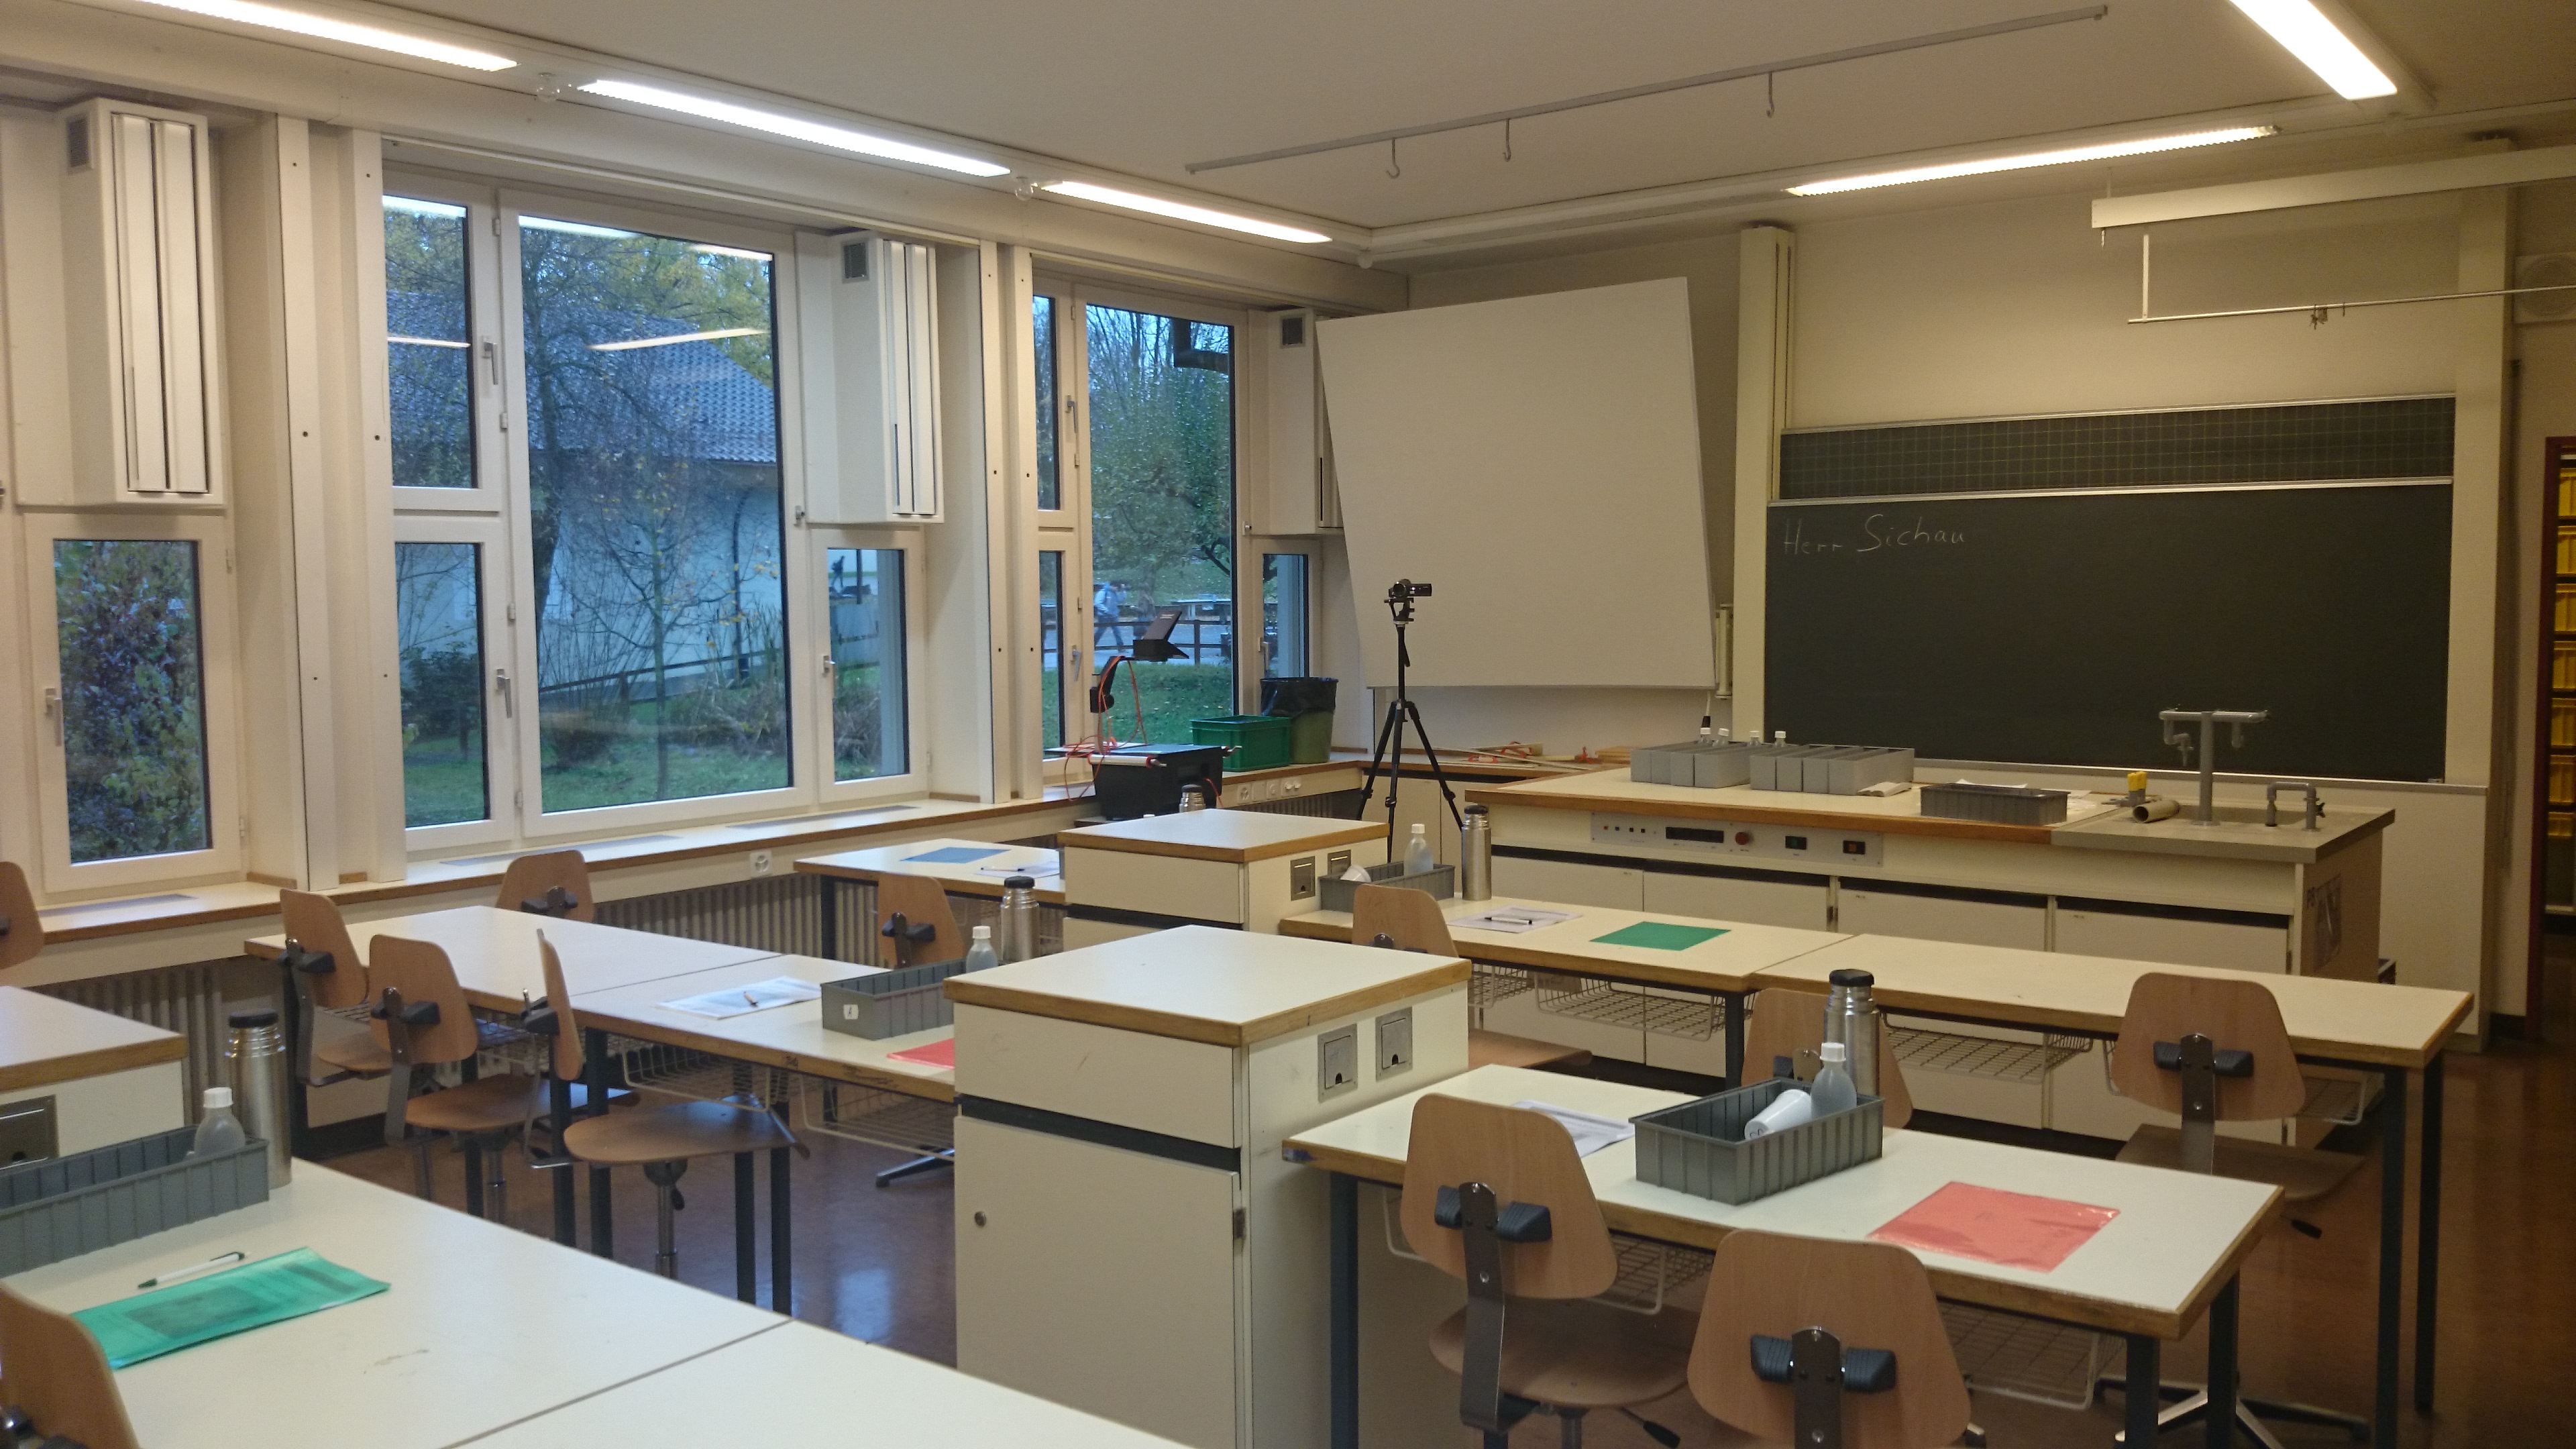
\includegraphics[width=0.7\linewidth]{graphics/Durchfuerhung}
\caption[Vorbereitetes Klassenzimmer.]{Klassenzimmer für die Durchführung des ersten Durchganges vorbereitet.}
\label{fig:Durchfuerhung}
\end{figure}

Zusätzlich wurden die Auswertungsbögen in der richtigen Reihenfolge und bereits mit einer Kodierung versehen, in einem Schnellhefter bereitgestellt. Ein für die Durchführung vorbereiteter Klassenraum ist im Bild \ref{fig:Durchfuerhung} ersichtlich.

Im Bild \ref{fig:Durchfuerhung} sieht man auch gut, wie die Kamera für die Videoaufwertung aufgestellt wurde. Die Videoaufnahme wurde bevor die Schülerinnen und Schüler den Klassenraum betreten haben gestartet, um die Ablenkung durch die Kamera möglichst gering zu halten.

\subsection{Durchführung}
Nachdem die Schülerinnen und Schüler in die beiden Räume aufgeteilt wurden, wurden Sie von den Versuchsleitern jeweils begrüsst. Die Begrüssung war stichwortartig vorbereitet, damit alle Klassen die gleichen Informationen erhielten und durch die Begrüssung die Testergebnisse nicht beeinflusst werden. Dabei wurde darauf hingewiesen, dass die Experimente keine Leistungskontrolle darstellt und alle Ergebnisse anonymisiert sind. Es wurde auch ein grober Überblick über den Ablauf gegeben. Im Raum in dem eine Videoaufnahme gemacht wurde, wurden die Schülerinnen und Schüler darüber informiert. 

Nach der Begrüssung wurden die Schülerinnen und Schüler aufgefordert mit den Tests anzufangen. Während der Zeit in welcher die Tests durchgeführt wurden, gaben die Versuchsleiter jeweils kurze Zeit Informationen und forderten die Schülerinnen und Schüler auf ihre Ergebnisse zu verschriftlichen.

Nach dem ersten Test (nach 20 Minuten) wurde eine Pause von fünf Minuten durchgeführt, in dieser wurden die Boxen ausgetauscht, sodass alle Schülerinnen und Schüler den nächsten hands-on Experimentiertest vor sich hatten. Die Schülerinnen und Schüler wurden aufgefordert sich innerhalb des Klassenraumes zu bewegen. Nach dem zweiten Test wurde eine grosse Pause durchgeführt, in welcher die Schülerinnen und Schüler das Schulzimmer verlassen hatten. Nach dem dritten Test wurde wieder eine kurze fünf-minütige Pause durchgeführt. Während den Test wurden den Schülerinnen und Schülern nur Fragen bei Unklarheiten beantwortet, inhaltliche Fragen oder Fragen zum korrekten Vorgehen wurden nicht beantwortet. 

\subsection{Nachbereitung}

Nachdem die Tests durchgeführt wurden, wurden die Auswertungsbögen eingesammelt und von David Sichau erst kodiert. Es wurde eine Zweitkodierung vor 15 \% der Auswertungsbögen von Pitt Hild durchgeführt. Die 11 Auswertungsbögen zur Zweit-Kodierung wurden per zufällig (random generator) ausgewählt, um sicherzugehen das ein Bias ausgeschlossen werden kann. Insgesamt wurden 72 Auswertungsbögen vollständig ausgefüllt. 

Die Videoaufnahmen wurden geschnitten, sodass nur noch die einzelnen Tests sichtbar sind. Dies wurde gemacht um zu vermeiden, dass Aktionen der Schülerinnen und Schüler in der Pause einen Einfluss auf die Bewertung in der Test Situation haben. Insgesamt ist Material zu 8 Schülerinnen und Schüler verwertbar, da die andern zu weit entfernt sind und daher ihre Aktionen nicht beobachtbar waren.


\chapter{Ergebnisse}
\section{Kodierung}

Wie bereits geschrieben wurde die Erstkodierung von David Sichau durchgeführt. Es wurden eine Zweitkodierung von  15 \% zufällig ausgewählten (per Random Generator) Auswertungsbögen von Pitt Hild  durchgeführt. Es wurden dabei die gleichen Kodierschemata verwendet, welche sich im Anhang der Arbeit befinden. %TODO Referenz zu Koderischemata

\subsection{Items}
Es gab insgesamt elf Items welche nach dem Kodierschemata kodiert wurden.

Die Items wurden auf Interrater-Reliabilität untersucht. Dafür wurden die prozedurale Übereinstimmung $p_0$ und zusätzlich noch das ungewichtete Cohen's Kappa $\kappa$ als Zufalls-korrigierter Koeffizient berechnet. Bei einem Teil der Datensätze war dies mathematisch nicht möglich (Division durch 0), daher können nicht für alle Items ein Cohen's Kappa angegeben werden. In Tabelle \ref{tab:CohenKappa} sind alle Ergebnisse zusammengefasst.


\github{http://git.io/mk9z-Q}

\begin{table}[htbp]
  \centering
\begin{tabular}{ccccccccc}
\toprule   &  \multicolumn{2}{c}{201} &&  \multicolumn{2}{c}{301}  && \multicolumn{2}{c}{301}\\
Item  & $p_0$ & $\kappa$ &&  $p_0$ & $\kappa$ &&  $p_0$ & $\kappa$\\
\midrule
 1.1 & 1 & 1  && 0.91 & 0.74 && 0.91 & 0.79 \\ 
 1.2 & 0.91 & 0.81  && 1 & /  && 1 & 1 \\ 
 2.1 & 0.81 & 0.67  && 0.81 & 0.74  && 1 & 1\\ 
 3.1 & 1 & 1  && 0.91 & 0.81  && 1 & 1\\ 
 3.2 & 1 & /  && 1 & 1  && 0.91 & 0.82\\ 
 4.1 & 0.91 & 0.79 && 0.81 & 0.65  && 0.91 & 0.81 \\ 
 4.2 & 0.91 & 0.62 && 0.91 & 0.79  && 0.91 & 0.74 \\ 
 4.3 & 1 & /  && 1 & /  && 1 & / \\ 
 4.4 & 1 & /  && 1 & /  && 1 & / \\ 
 5.1 & 1 & /  && 1 & /  && 1 & / \\ 
 5.2 & 0.91 & /  && 1 & 1  && 0.91 & 0.78 \\ 

\bottomrule

\end{tabular} 
  \caption{Übereinstimmung der Kodierungen für die einzelnen Items ($p_0$) und Cohens Kappa $\kappa$. Für die drei Tests 201 (Chemie-Temperatur), 301 (Physik Kraft) und 305 (Physik Temperatur)}
  \label{tab:CohenKappa}
\end{table}

\subsection{Qualitätsstandards}
Aus den elf Items wurden fünf Qualitätsstandards entwickelt \citep{Hild2014a}. Es gibt bedingte und unbedingte Qualitätsstandards. Bei den bedingten Qualitätsstandards ist für das erreichen notwendig, das sowohl die Bedingung erfüllt ist, als auch dass der vorgängige Qualitätsstandard erfüllt ist. Die unbedingten Qualitätsstandards werden in dieser Arbeit mit Q1 bis Q5 bezeichnet. Die bedingten Qualitätsstandards werden mit QS1 bis QS5 bezeichnet.
\subsubsection*{Qualitätsstandard 1}
Im Qualitätsstandard 1 geht es um das korrekte und präzise messen. Dieser Qualitätsstandard wird nur erreicht wenn Item 1.1 (Richtige Tendenz des Resultates) und Item 1.2 (Ist das Resultat vollständig und korrekt) zusammen mindestens 1 ergeben.


\subsubsection*{Qualitätsstandard 2}
Bei Qualitätsstandard 2 wird die Dokumentation der Messung bewertet . Dieser Qualitätsstandard wird nur erreicht wenn Item 1.2 (Werden alle Messungen und Messergebnisse vollständig dargestellt) mindestens den Wert von 2 erreicht hat. 

\subsubsection*{Qualitätsstandard 3}
Im dritten Qualitätsstandard wird das Begründen des richtigen Messinstrumentes bewertet. Dieser Standard wird nur erreicht wenn Item 3.1 (Ist das Korrekte Messinstrument gewählt worden) und Item 3.2 (Wird die Wahl des Messinstrumentes korrekt begründet) zusammen zwei ergeben.

\subsubsection*{Qualitätsstandard 4}
Qualitätsstandard 4 beurteilt die Messwiederholung. Es wird aus Item 4.1 (mehrmaliges Messen), 4.2 (identische Messung), 4.3 (wurde Mittelwert gebildet) und 4.4 (korrekter Mittelwert) gebildet. Diese Level wird erreicht wenn die Items addiert mindestens zwei ergeben.

\subsubsection*{Qualitätsstandard 5}
Der letzte Qualitätsstandard 5 zeigt auf, inwiefern die Schülerinnen und Schüler Fehlerquellen der Messung begründen können. Dieser Standard besteht aus Item 5.1 (Fehlerkategorien nennen) und 5.2 (Verbesserungsvorschläge) welche zusammen mehr als eins ergeben müssen.

\subsubsection{Erreichte Qualitätsstandards}

In Tabelle \ref{tab:QS} wird ein Überblick über die erreichten Qualitätsstandards aller Schülerinnen und Schüler gegeben. Zusätzlich werden auch die bedingten Qualitätsstandards angeben, welche nur erreicht werden können, wenn der vorhergehende Qualitätsstandard erreicht wurde.


\begin{table}[!htbp]
  \centering
\begin{tabular}{ccccccccccc}
\toprule
 Test & $p_{Q1}$ & $p_{QS1}$ & $p_{Q2}$ & $p_{QS2}$& $p_{Q3}$& $p_{QS3}$& $p_{Q4}$& $p_{QS4}$& $p_{Q5}$& $p_{QS5}$\\ 
\midrule
 201 &   0.51 & 0.51& 0.34 & 0.27 & 0.05 & 0.04 & 0.08 & 0.03 & 0.16 & 0.03 \\ 
 301 &   0.62 & 0.62& 0.31 & 0.31 & 0.09 & 0.04 & 0.09 & 0.01 & 0.39 & 0.01\\ 
 305 &   0.72 & 0.72& 0.30 & 0.29 & 0.35 & 0.14 & 0.11 & 0.01 & 0.50 & 0.01\\ 
\bottomrule
\end{tabular} 
  \caption{Zusammenfassung der erreichten Qualitätsstandards, wobei $p_{Q1} - p_{Q5}$ den unbedingten Qualitätsstandards entsprechen. Die bedingten Qualitätsstandards werden mit $p_{QS1} - p_{QS5}$ bezeichnet.}
  \label{tab:QS}
\end{table}




\subsection{Niveau}

Basierend auf den Qualitätsstandards wurden zwei Niveaus gebildet, welche das erreichte Niveau der Schülerinnen und Schüler bei der Kompetenz des skalenbasierten Messens bezeichnen. Die Niveaus können einen Wert zwischen 0 und 5 annehmen. Eine Übersicht über die erreichten Niveaus wird in Tabelle \ref{tab:Niveau} gegeben.
\github{http://git.io/bjn9qg}

\begin{table}[htbp]
  \centering
\begin{tabular}{cccccccccccccc}
\toprule
 &  \multicolumn{6}{c}{uLev} &&  \multicolumn{6}{c}{kLev}\\ 
 Test & 0 & 1 & 2 & 3 & 4 & 5 && 0 & 1 & 2 & 3 & 4 & 5\\ 
\midrule
 201 &   0.36 & 0.24 & 0.22 & 0.13 & 0.03 & 0.03 && 0.40 & 0.24 & 0.32  & 0.01 & 0 & 0.03   \\ 
 301 &   0.31 & 0.21 & 0.29 & 0.14 & 0.03 & 0.03  && 0.42 & 0.28 & 0.26 & 0.01 & 0 & 0.03  \\ 
 305 &   0.13 & 0.19 & 0.24 & 0.31 & 0.11 & 0.03  && 0.22 & 0.43 & 0.18 & 0.13 & 0.01 & 0.03 \\ 
\bottomrule
\end{tabular} 
  \caption{Prozedural erreichte Niveaus aller Schülerinnen und Schüler. Das unbedingte Niveau wird mit uLev und das bedingte Niveau mit kLev bezeichnet. }
  \label{tab:Niveau}
\end{table}

\subsubsection{Unbedingtes Niveau}
Dieses Niveau ist der Summenscore der einzelnen unbedingten Qualitätsstandards. In der Arbeit wird dieses Level mit \textit{uLev} abgekürzt.

\subsubsection{Bedingtes Niveau}

Dieses Niveau ist der Summenscore der bedingten Qualitätsstandards. Dieses Niveau wird mit \textit{kLev} abgekürzt.




\section{Fragebogen}

Im standardisierten Teil des Fragebogens wurden Fragen zum absoluten Selbstkonzept nach SESSKO gestellt \citep{Schone2002}. Die verwendeten Fragen sind in Tabelle \ref{tab:SESSKO} aufgeführt. 



\begin{table}[htbp]
  \centering
\begin{tabular}{p{3cm}p{9cm}p{1cm}}
\toprule Skala & Frage & $\alpha_d$  \\ 
\midrule SESSKO 18(a) & Ich bin für die Schule sehr begabt. &  0.71  \\ 
 SESSKO 19(a) & Neues zu lernen fällt mir schwer.  &  0.76 \\ 
 SESSKO 20(a) & Ich bin sehr intelligent. &  0.71  \\ 
 SESSKO 21(a) & Ich kann in der Schule viel. &  0.72   \\ 
 SESSKO 22(a) & In der Schule fallen mir viele Aufgaben schwer.  & 0.74   \\ 
\bottomrule 
\end{tabular} 
  \caption{Fragen von SESSKO zur Skala "`Schulisches Selbstkonzept - absolut"'  \citep{Schone2002}. $\alpha_d$ bezeichnete das standardisierte Cronbach Alpha wenn dieses Item weggelassen würde.}
  \label{tab:SESSKO}
\end{table}

Zusätzlich wurden nach \citet{Dierks2014} Fragen zum Selbstkonzept zu Schulversuchen entwickelt und angepasst. Die entwickelten Fragen sind in Tabelle \ref{tab:NatSK} aufgezeigt.

\begin{table}[htbp]
  \centering
\begin{tabular}{p{2cm}p{10cm}p{1cm}}
\toprule Kürzel & Frage & $\alpha_d$  \\ 
\midrule NatSK1 & Schulversuche liegen mir nicht besonders. &  0.65  \\ 
 NatSK2 & Schulversuche würde ich viel lieber machen, wenn sie nicht so schwer wären.  &  0.69 \\ 
 NatSK3 & Schulversuche fallen mir schwerer als vielen meiner Mitschüler/innen. &  0.65  \\ 
 NatSK4 & Bei manchen Schulversuche weiss ich gleich: "`Das verstehe ich nie."' &  0.65   \\ 
 NatSK5 & Für Schulversuche habe ich einfach keine Begabung.   & 0.63   \\ 
 NatSK6 & Mit den Aufgaben bei Schulversuche komme ich besser zurecht als viele meiner Mitschüler/innen  & 0.67   \\ 
 NatSK7 & Ich denke, ich bin für Schulversuche begabter als viele meiner Mitschüler/innen.  & 0.66   \\ 
\bottomrule 
\end{tabular} 
  \caption{Fragen zum Sebstkonzept bei Schulversuchen abgewandelt nach \citet{Dierks2014}. $\alpha_d$ bezeichnete das standardisierte Cronbach Alpha wenn dieses Item weggelassen würde.}
  \label{tab:NatSK}
\end{table}

Es wurde die innere Konsistenz beider Skala überprüft. Bei den der Skala "`Schulisches Selbstkonzept - absolut"' wurde ein standardisiertes Cronbach $\alpha$ von 0.77 erreicht. Die Anzahl vollständig ausgefüllter Fragebögen betrug dabei 69. Alle unvollständigen Items wurden vor der Analyse entfernt. Bei der Skala zum Selbstkonzept bei Schulversuchen wurde ein standardisiertes Cronbach $\alpha$ von 0.69 erreicht. Insgesamt konnten dabei 64 vollständige Fragebögen ausgefüllt werden. 
\github{http://git.io/WyJH6Q}


\section{Unterschiede zwischen den Klassen}

Um festzustellen, ob alle Datensätze der einzelnen Klassen kombiniert werden dürfen wurden zuerst alle Klassen einzeln gegeneinander auf folgende Nullhypothese überprüft: 
\begin{quote}
Besteht \underline{kein} Unterschied in den Qualitätsstandards zwischen den einzelnen Klassen?
\end{quote}
Es wurden dabei die Qualitätsstandards verglichen, da diese im Vergleich zu den Items ein geringeres Rauschen aufweisen, ohne jedoch gross an Informationsgehalt eingebüsst zu haben.


Aufgrund der geringen Anzahl an Beobachtungen für einzelne Qualitätsstandards wurde der exakter Test nach Fisher verwendet. Es wurden Kontingenztafeln für jeden Qualitätsstandard (Q1 bis Q5 und QS1 bis QS5) erstellt und in jeder Tafel die beiden Levels (0 und 1) gegenüber den Klassen verglichen.


\begin{table}[htbp]
  \centering
\begin{tabular}{cccccccccccccc}
\toprule
 Klasse & Q1 & Q2 & Q3 & Q4 & Q5 && QS1 & QS2 & QS3 & QS4 & QS5 \\ 
\midrule
 1 vs. 2 &   0.68 & 1.00 & 1.00 & 0.60 & 1.00 && 0.51 & 0.59 & 1.00 & 1.00 & 1.00   \\ 
 1 vs. 3 &   1.00 & 0.72 & 1.00 & 1.00 & 1.00 && 1.00 & 0.72 & 1.00 & 1.00 & 1.00   \\
 1 vs. 4 &   0.43 & 0.72 & 0.22 & 0.32 & 0.65 && 0.42 & 0.72 & 0.48 & 1.00 & 1.00   \\
 2 vs. 3 &   0.68 & 0.72 & 1.00 & 0.22 & 1.00 && 0.68 & 1.00 & 1.00 & 1.00 & 1.00   \\
 2 vs. 4 &   1.00 & 0.72 & 0.60 & 1.00 & 1.00 && 1.00 & 1.00 & 1.00 & 1.00 & 1.00   \\
 3 vs. 4 &   0.43 & 1.00 & 0.22 & 0.10 & 0.65 && 0.43 & 1.00 & 0.48 & 1.00 & 1.00   \\
\bottomrule
\end{tabular} 
  \caption{p-Werte für den exakten Test nach Fisher für die Vergleiche der einzelnen Klassen untereinander auf allen Qualitätsstandards. Kein p-Wert in dieser Tabelle liegt unter 0.05. }
  \label{tab:KlassenVergleiche}
\end{table}


Die Resultate des exakten Tests nach Fisher befindet sich in Tabelle \ref{tab:KlassenVergleiche}. Bei keinem der 60 Tests konnte die Nullhypothese abgelehnt werden (p<0.05). Daher gibt es keinen signifikanten Unterschied zwischen den erreichten Qualitätsstandards in den einzelnen Klassen.  
\github{http://git.io/0DOelQ}

\section{Korrelation der Niveaus des skalenbasierten Messens}

In einem nächsten Schritt wurde untersucht inwiefern die Niveau-Stufen (uLev und cLev) zwischen den einzelnen Tests korrelieren. Dazu wurde als Rangkorrelationskoeffizient Spearmans $\rho$ berechnet. Der Vorteil dieser Methode ist, dass keine Annahmen über die Zugrundliegeenden Daten gemacht werden muss. Des Weiteren bietet diese Methode den Vorteil, dass sie gegenüber Ausreissern robust ist. 

Da die Korrelation alleine keinen Aufschluss darüber gibt, ob diese Korrelation signifikant ist, wurde die Korrelation zusätzlich auf Signifikanz getestet. Wichtig bei dieser Analyse ist, dass die Korrelation keine Aussage über die Kausalität zulässt.


Die Ergebnisse wurden grafisch als Streudiagramme dargestellt (siehe \ref{fig:corLev}). In die Streudiagramme wurde die Gerade der linearen Regression eingetragen mit dem zugehörigen 95\% Vertrauensintervall. Zusätzlich wurde die noch Spearmans $\rho$ und der p-Wert des Signifikanztests angegeben, diese Werte sind auch in Tabelle \ref{tab:CorNiveau} zusammengefasst.



\begin{table}[htbp]
  \centering
\begin{tabular}{ccccccc}
\toprule
 &&  \multicolumn{2}{c}{uLev} &&  \multicolumn{2}{c}{kLev}\\ 
 Test && p-Wert & $\rho$ && p-Wert & $\rho$  \\ 
\midrule
 201 vs. 301 &&   0.02 & 0.26 && 0.20 & 0.08    \\ 
 201 vs. 305 &&   0.44 & 1e-4 && 0.33 & 4e-3      \\
 301 vs. 305 &&   0.36 & 2e-3 && 0.01 & 0.89    \\
\bottomrule
\end{tabular} 
  \caption{Spearmans $\rho$ und p-Werte für die Korrelation zwischen den unbedingten Niveaus (uLev) und den bedingten Niveaus (kLev) zwischen den einzelnen Tests.  }
  \label{tab:CorNiveau}
\end{table}
 
\begin{figure}[bhtp]
\centering
\begin{subfigure}{0.49\textwidth}
  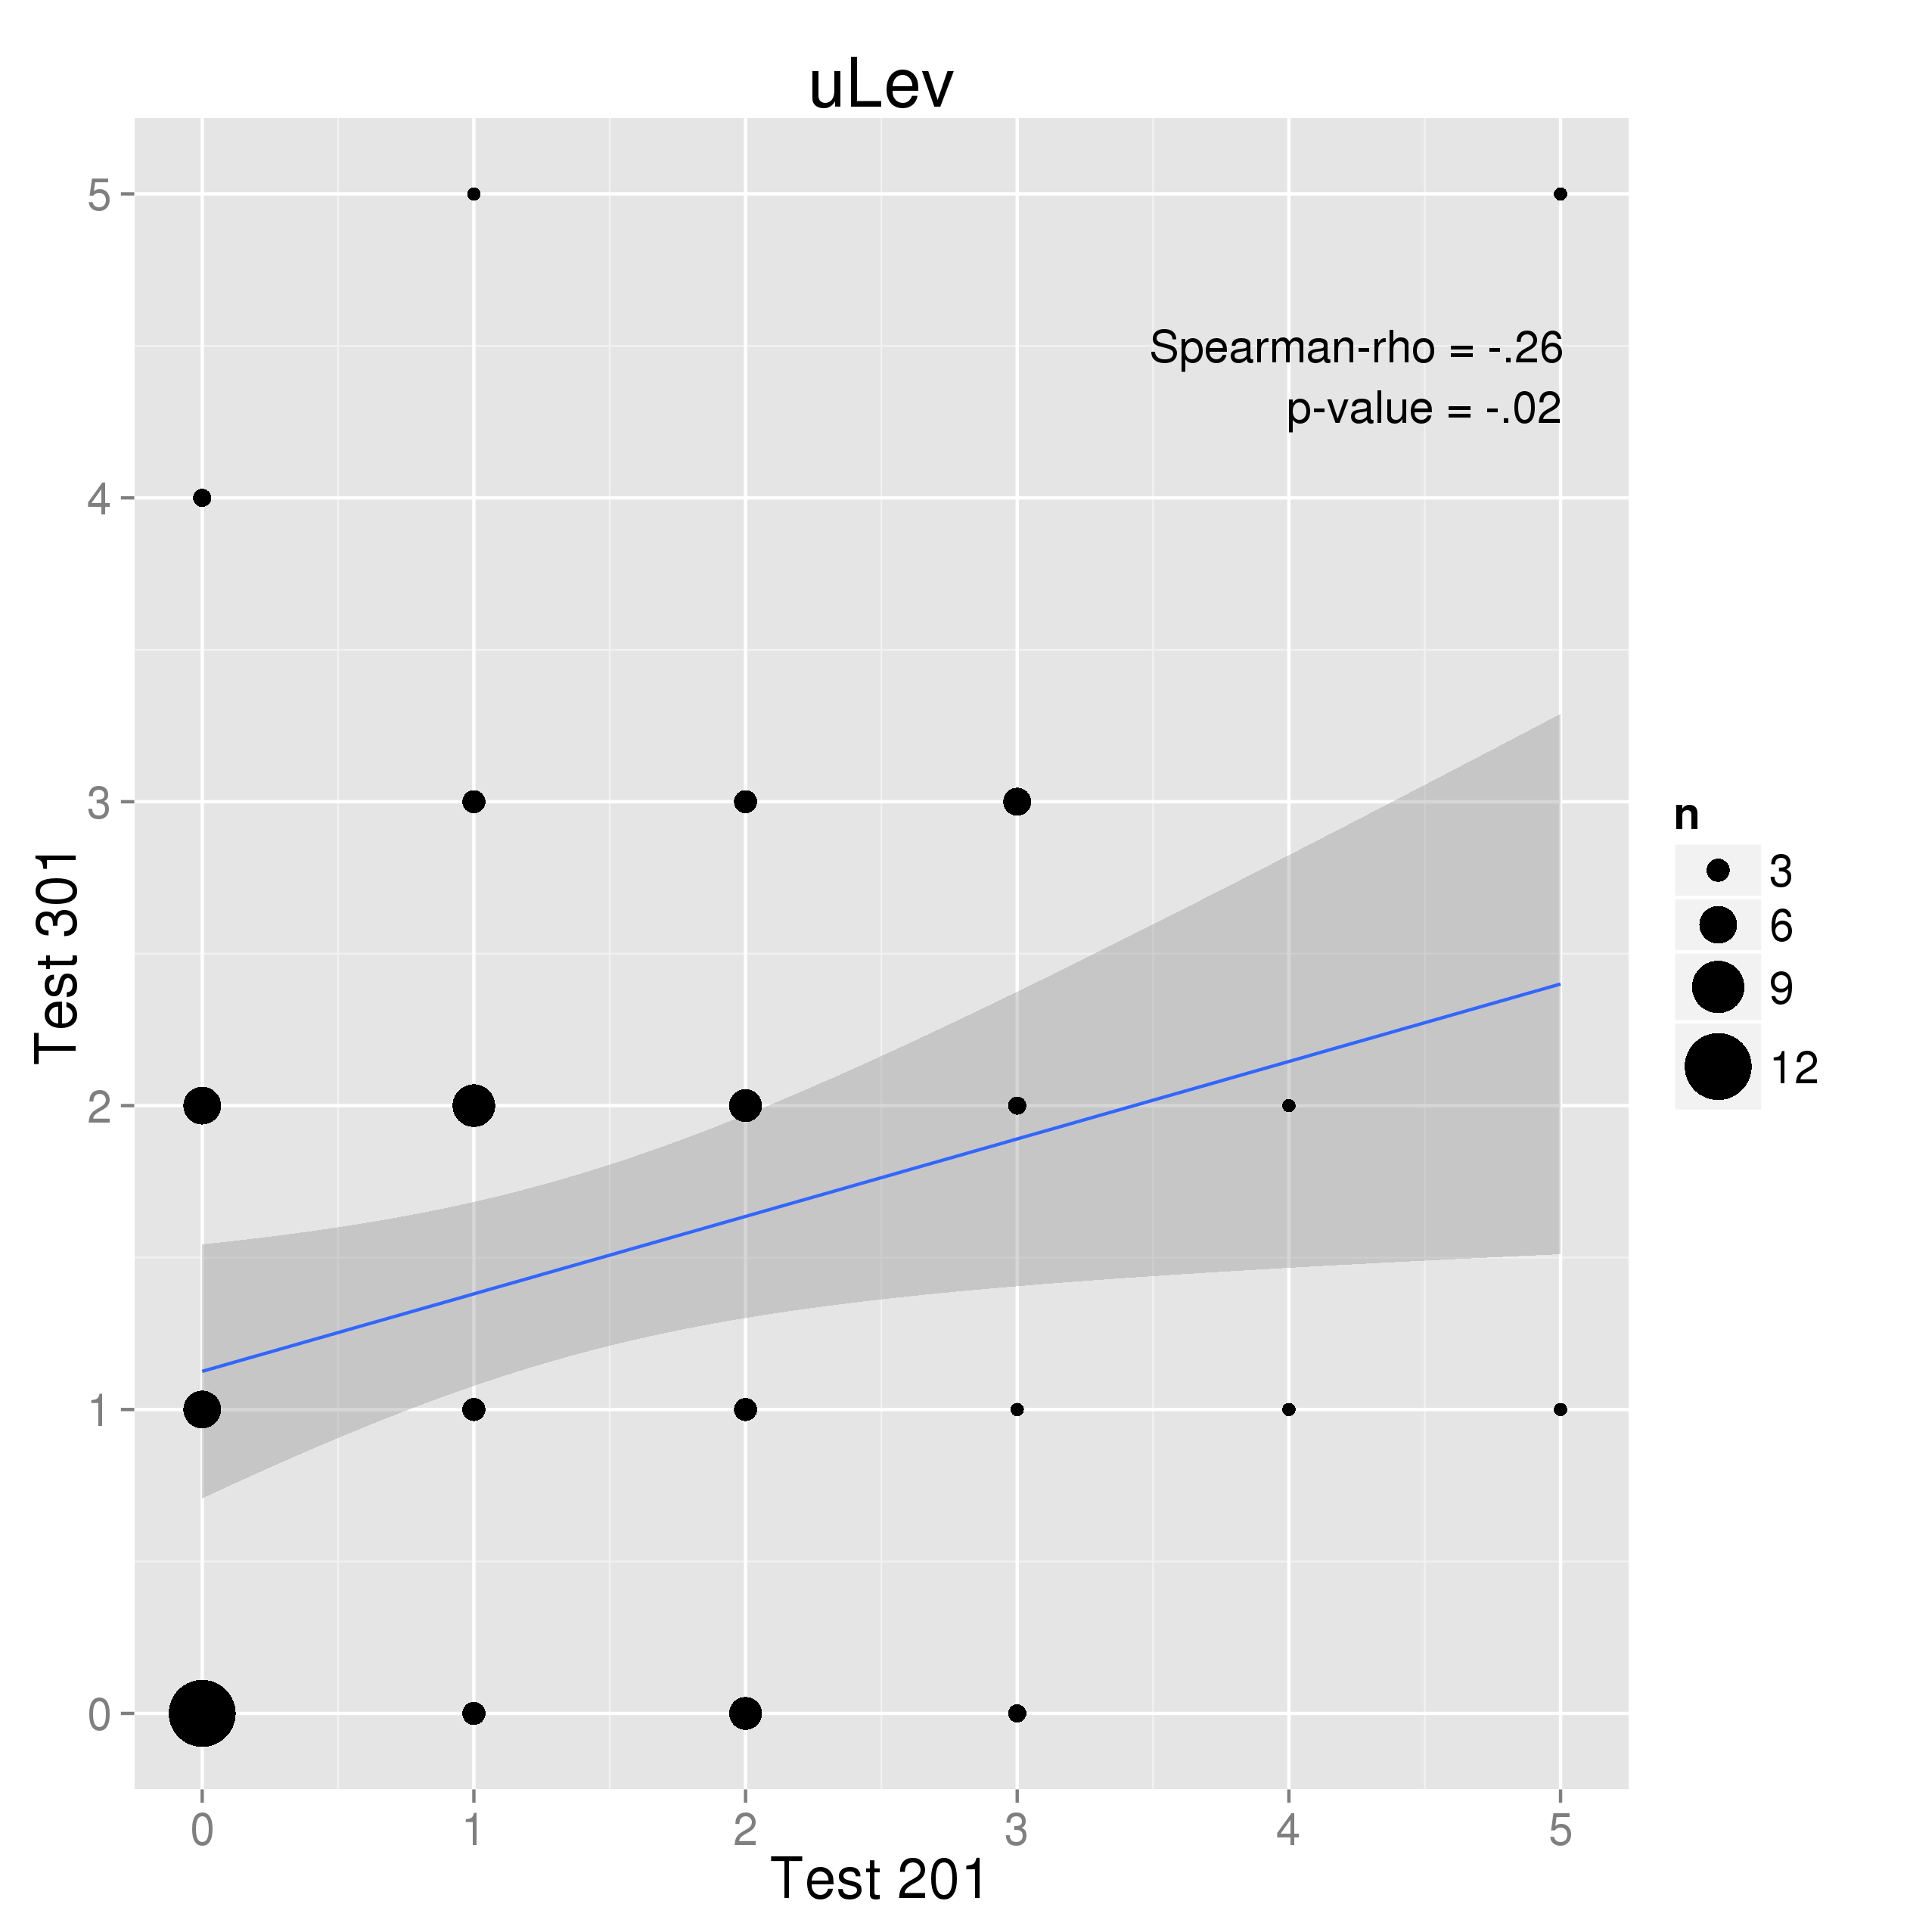
\includegraphics[width=1.0\linewidth]{graphics/cor201301u.png}
  \caption{unbedingte Niveau-Stufen}
  \label{fig:cor201301k}
\end{subfigure}
\begin{subfigure}{0.49\textwidth}
  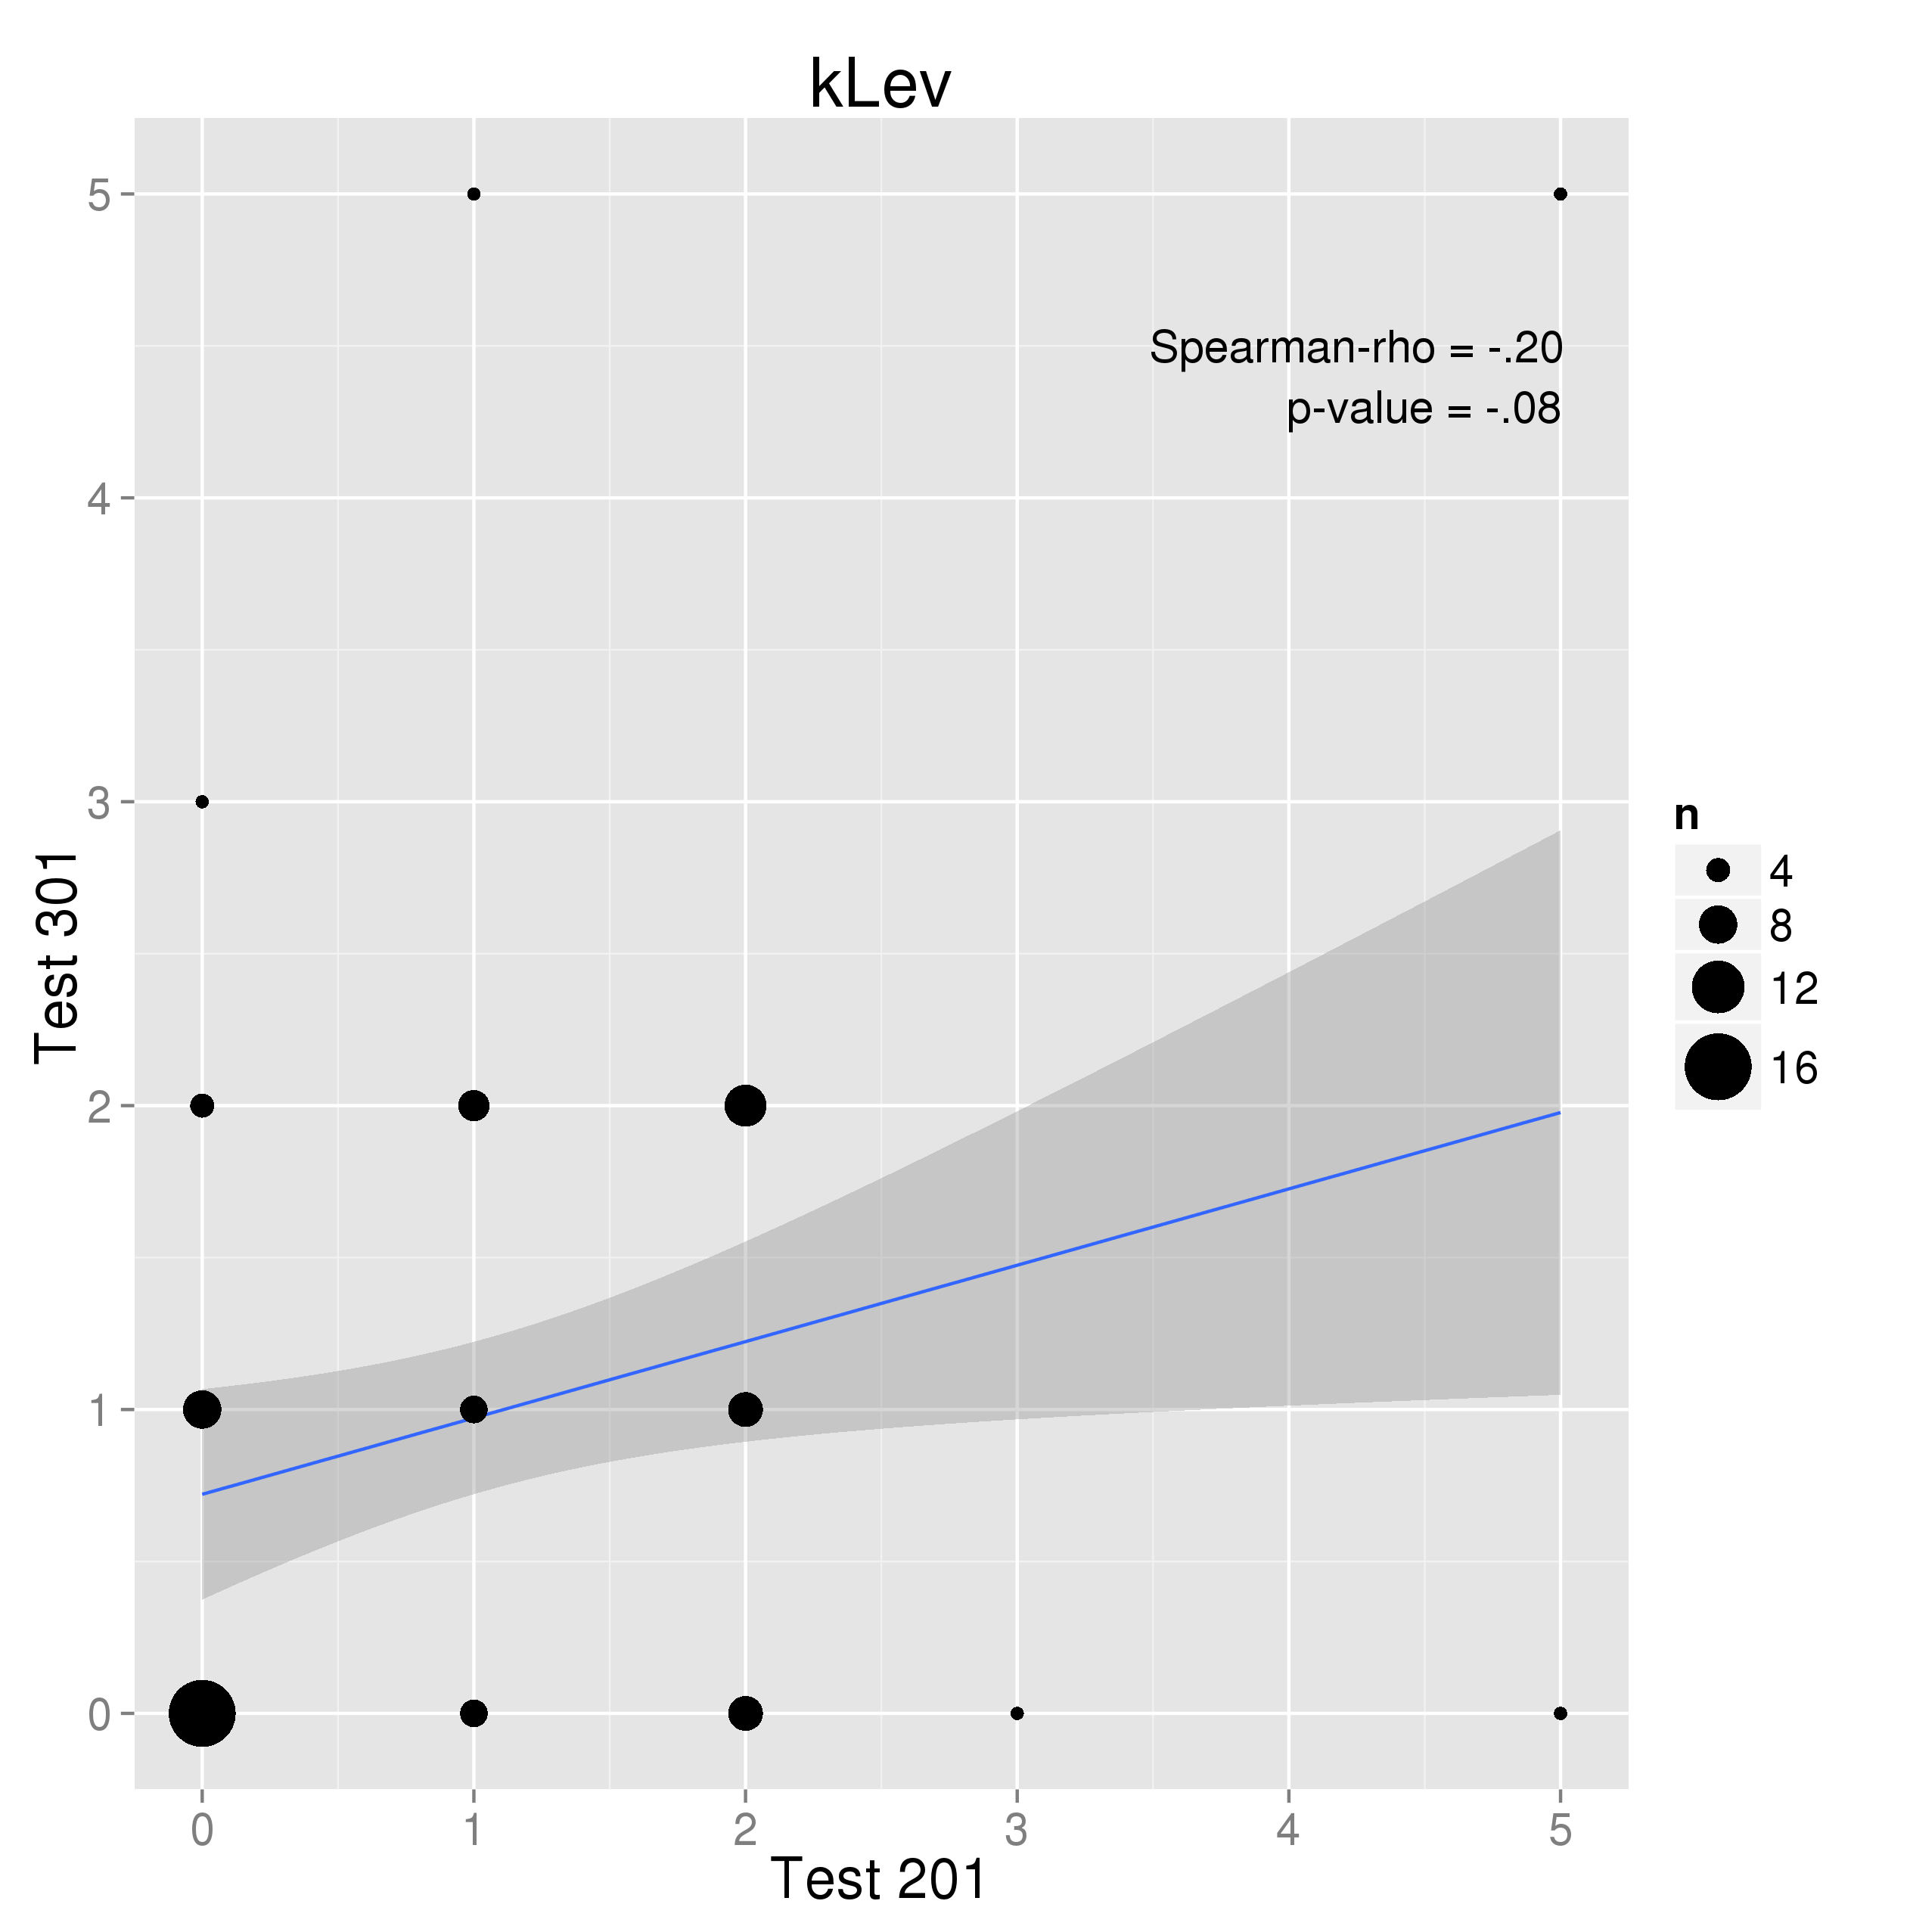
\includegraphics[width=1.0\linewidth]{graphics/cor201301k.png}
  \caption{bedingte Niveau-Stufen}
  \label{fig:cor201301u}
\end{subfigure}
\end{figure}
\begin{figure}[htbp]
\ContinuedFloat % continue from previous page
\centering
\begin{subfigure}{0.49\textwidth}
  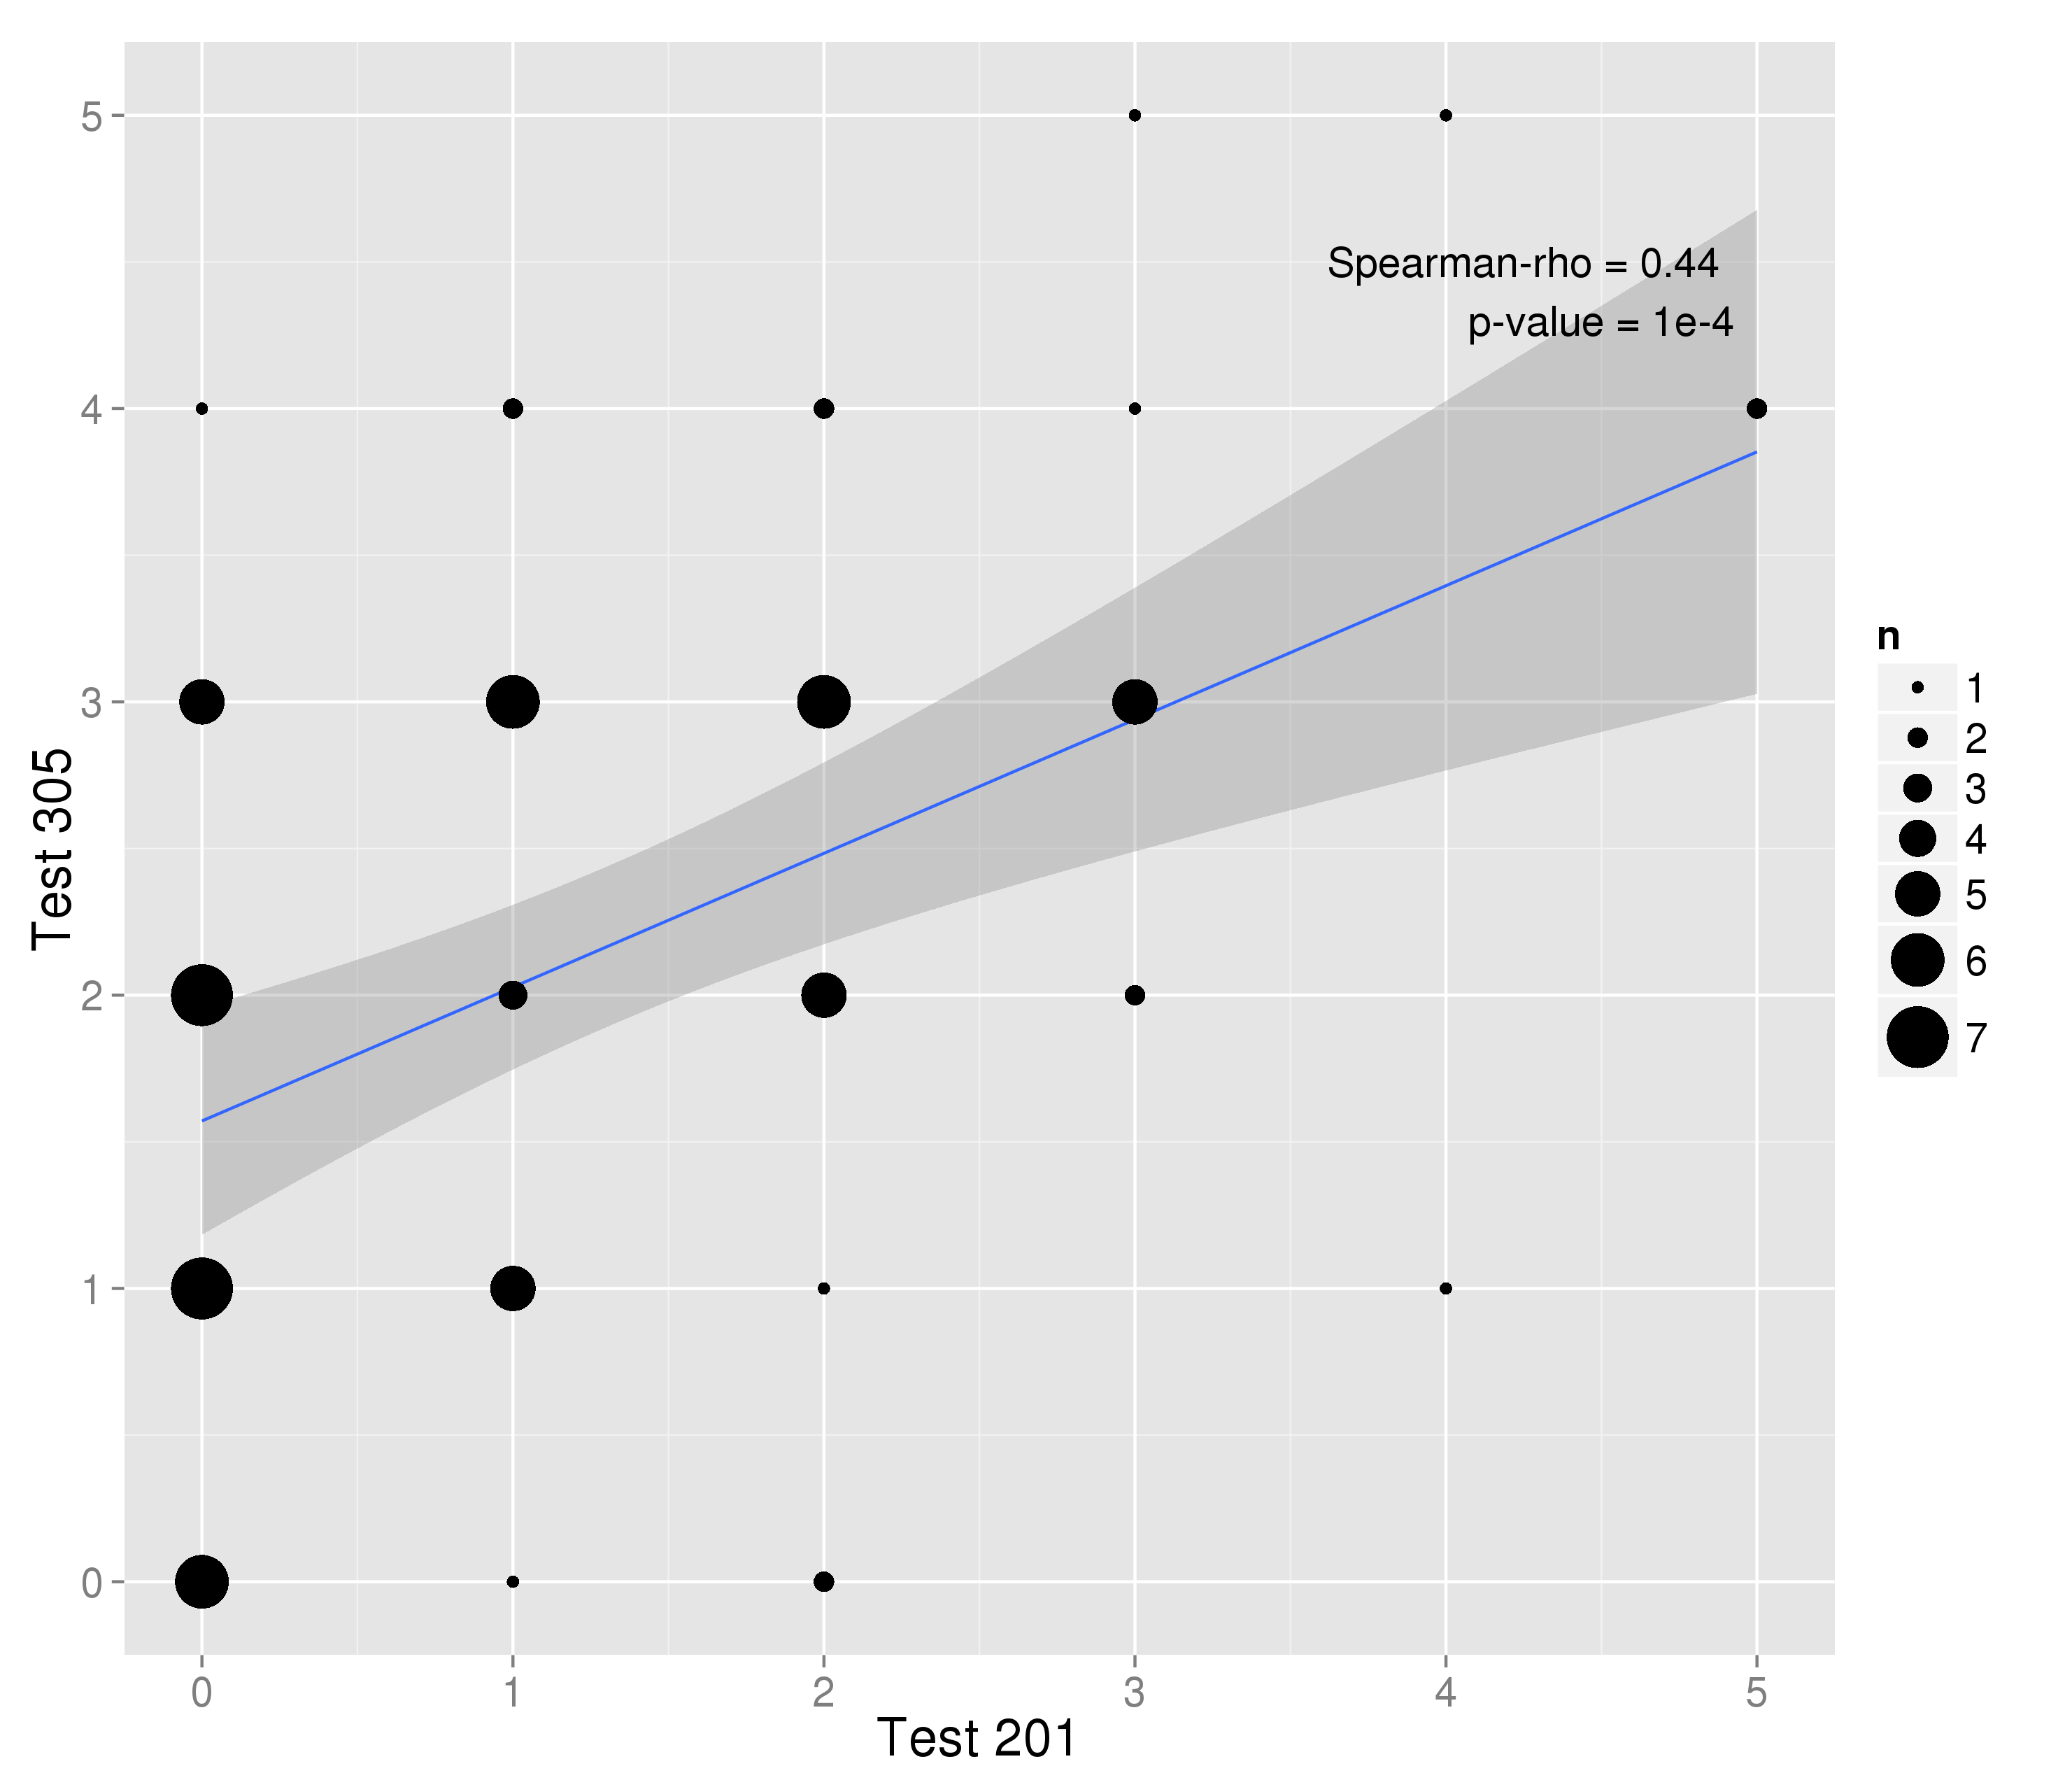
\includegraphics[width=1.0\linewidth]{graphics/cor201305u.png}
  \caption{unbedingte Niveau-Stufen}
  \label{fig:cor201305k}
\end{subfigure}
\begin{subfigure}{0.49\textwidth}
  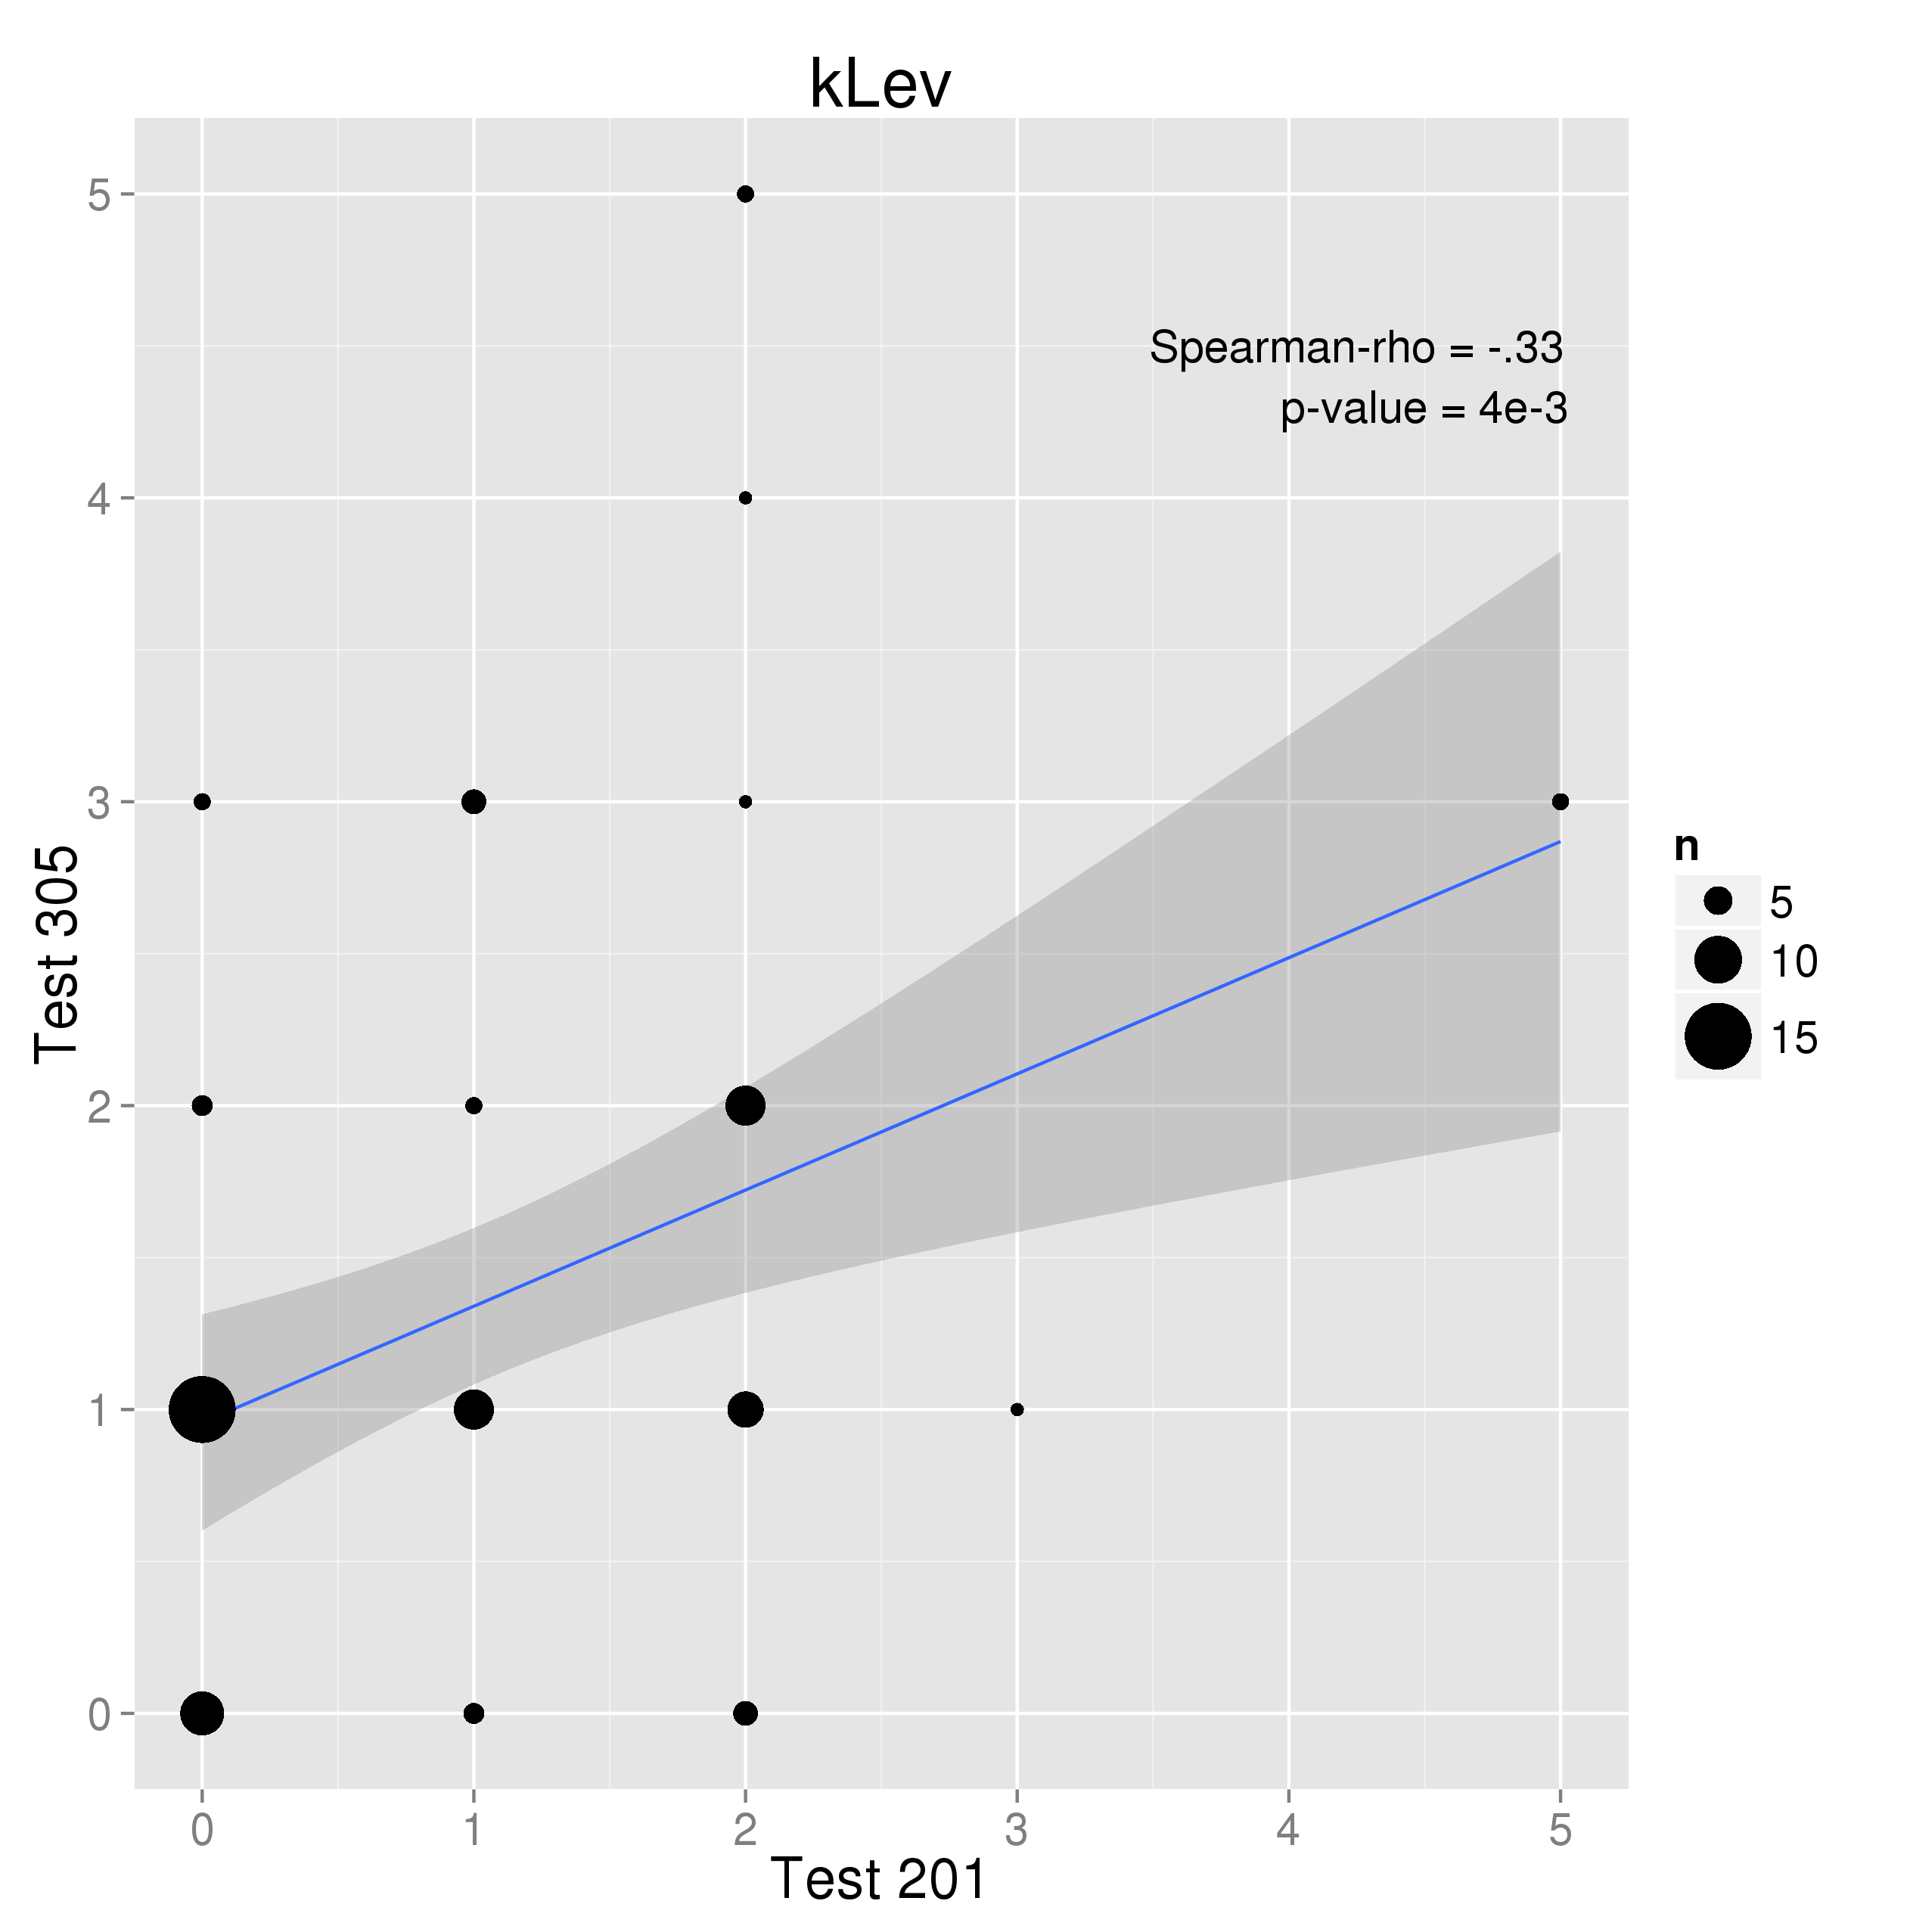
\includegraphics[width=1.0\linewidth]{graphics/cor201305k.png}
  \caption{bedingte Niveau-Stufen}
  \label{fig:cor201305u}
\end{subfigure}
\end{figure}
\begin{figure}[htbp]
\ContinuedFloat % continue from previous page
\centering
\begin{subfigure}{0.49\textwidth}
  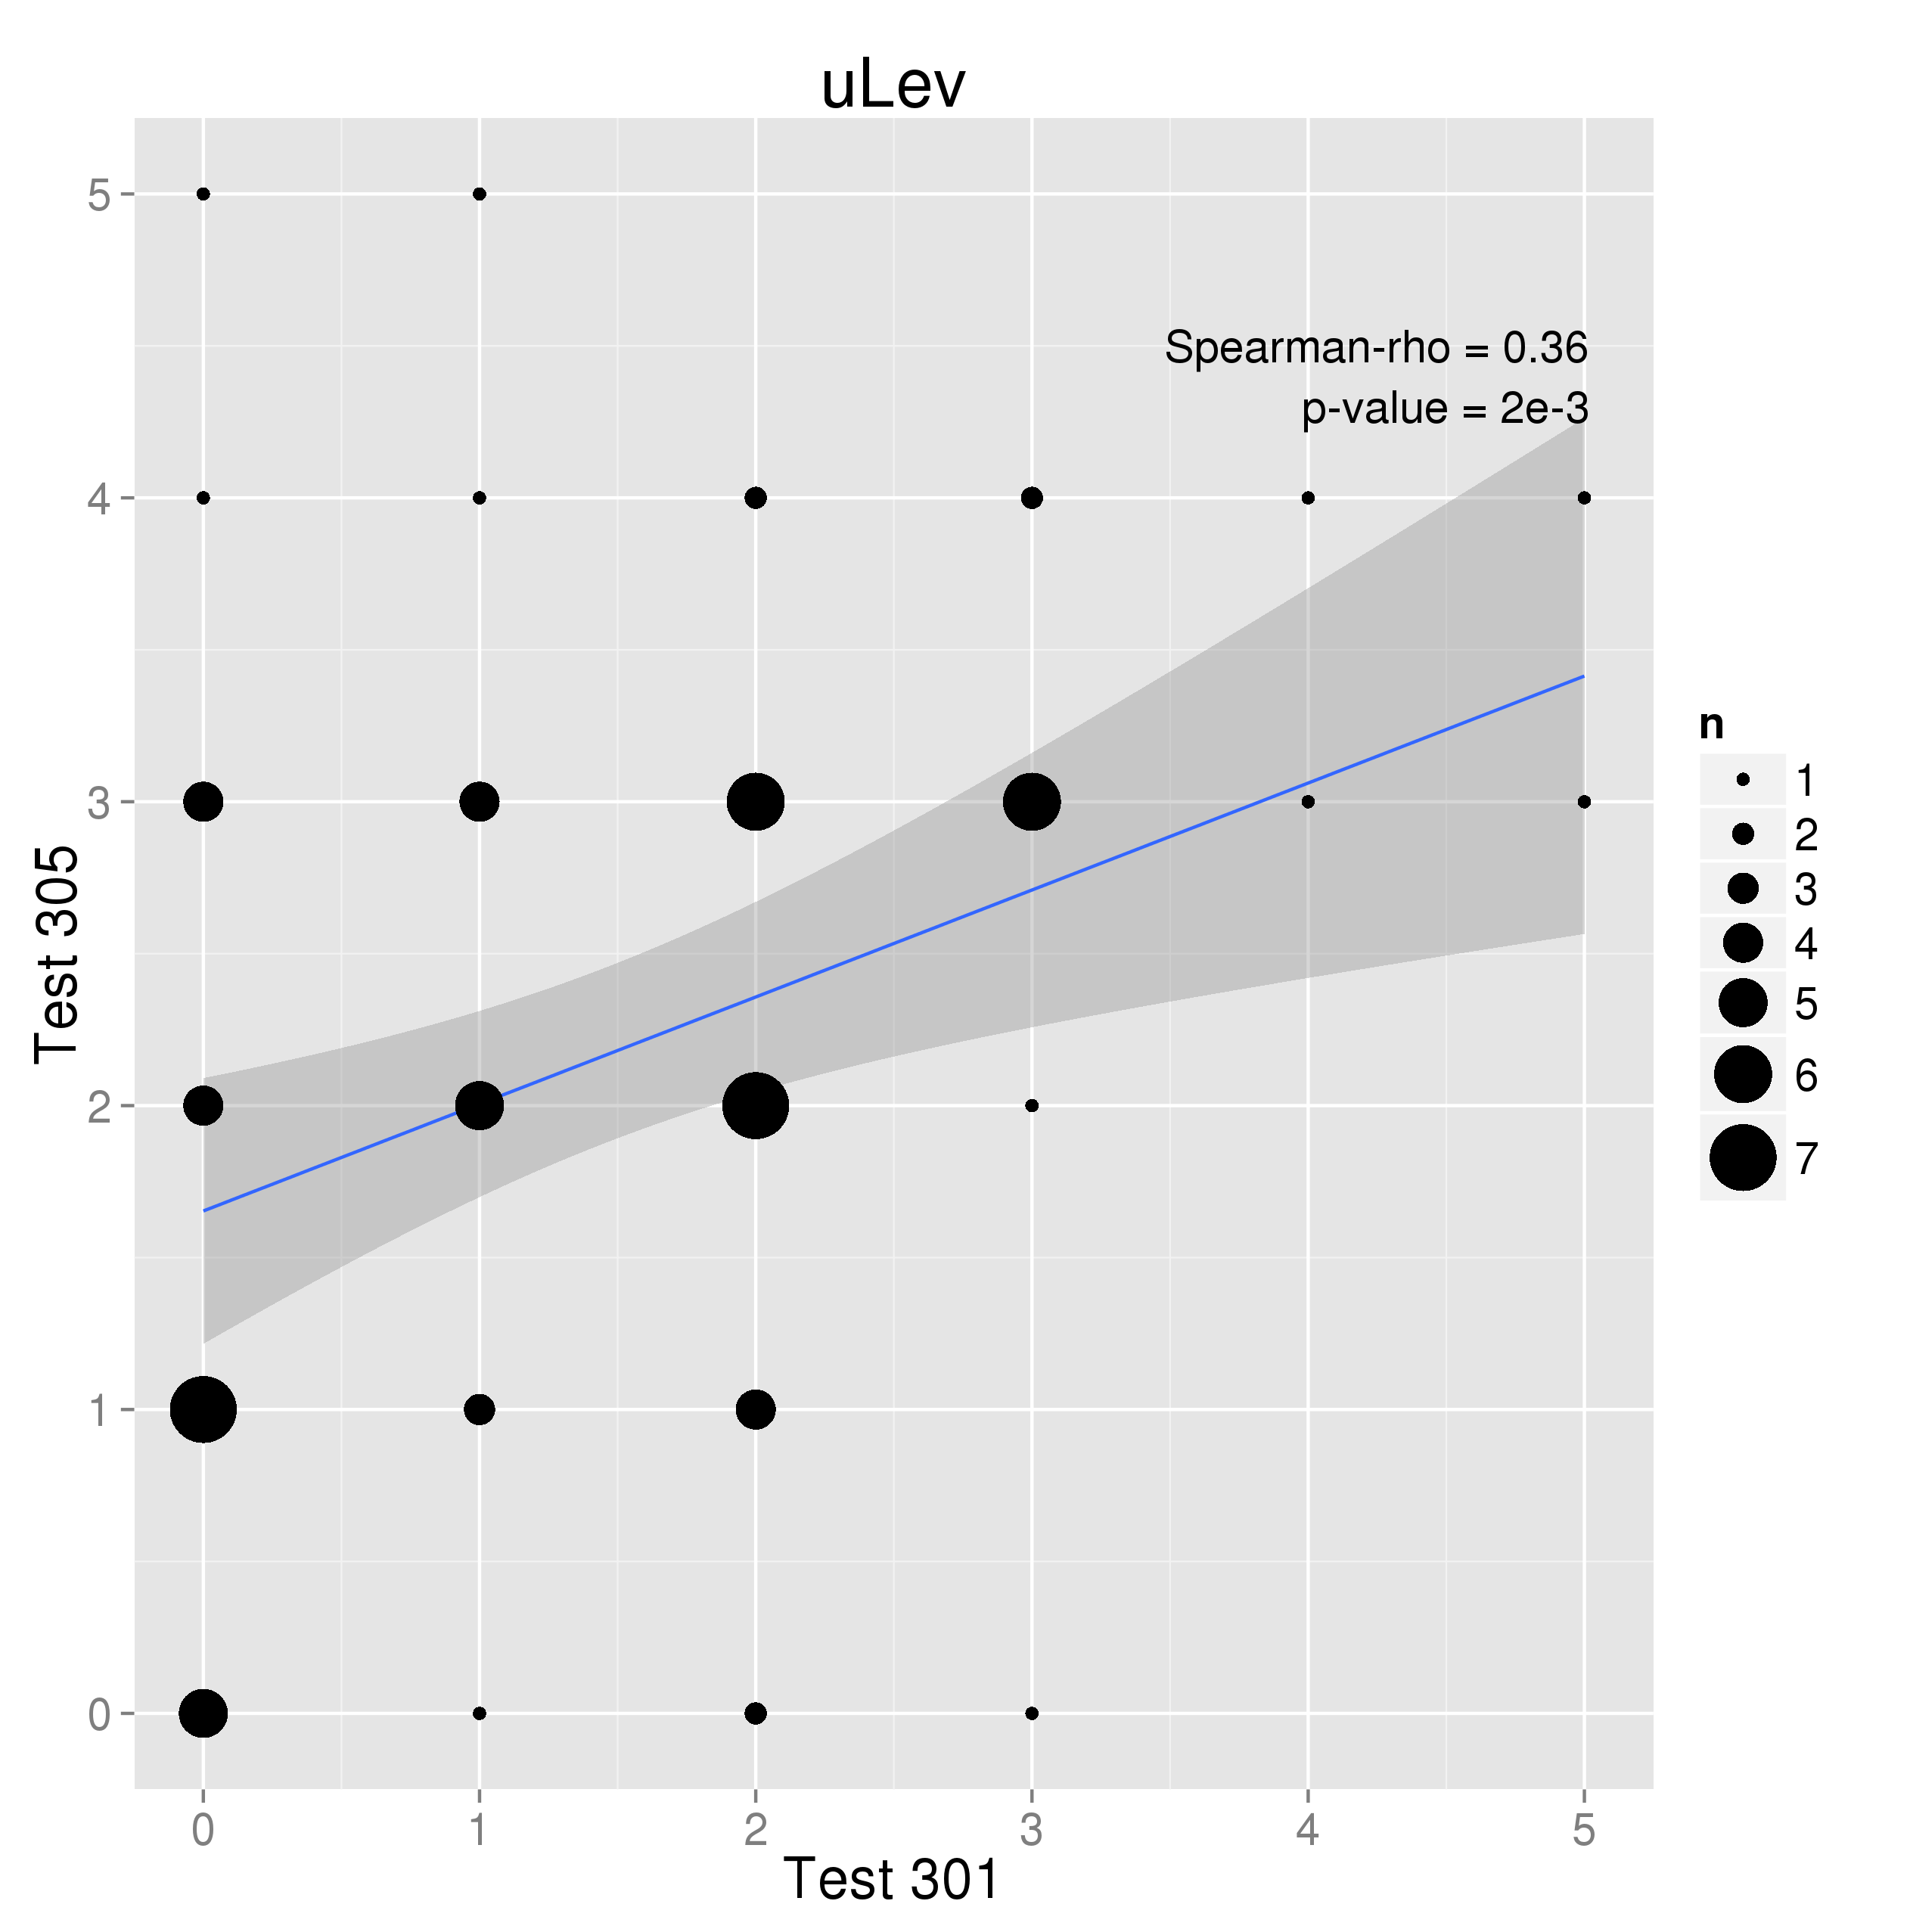
\includegraphics[width=1.0\linewidth]{graphics/cor301305u.png}
  \caption{unbedingte Niveau-Stufen}
  \label{fig:cor301305k}
\end{subfigure}
\begin{subfigure}{0.49\textwidth}
  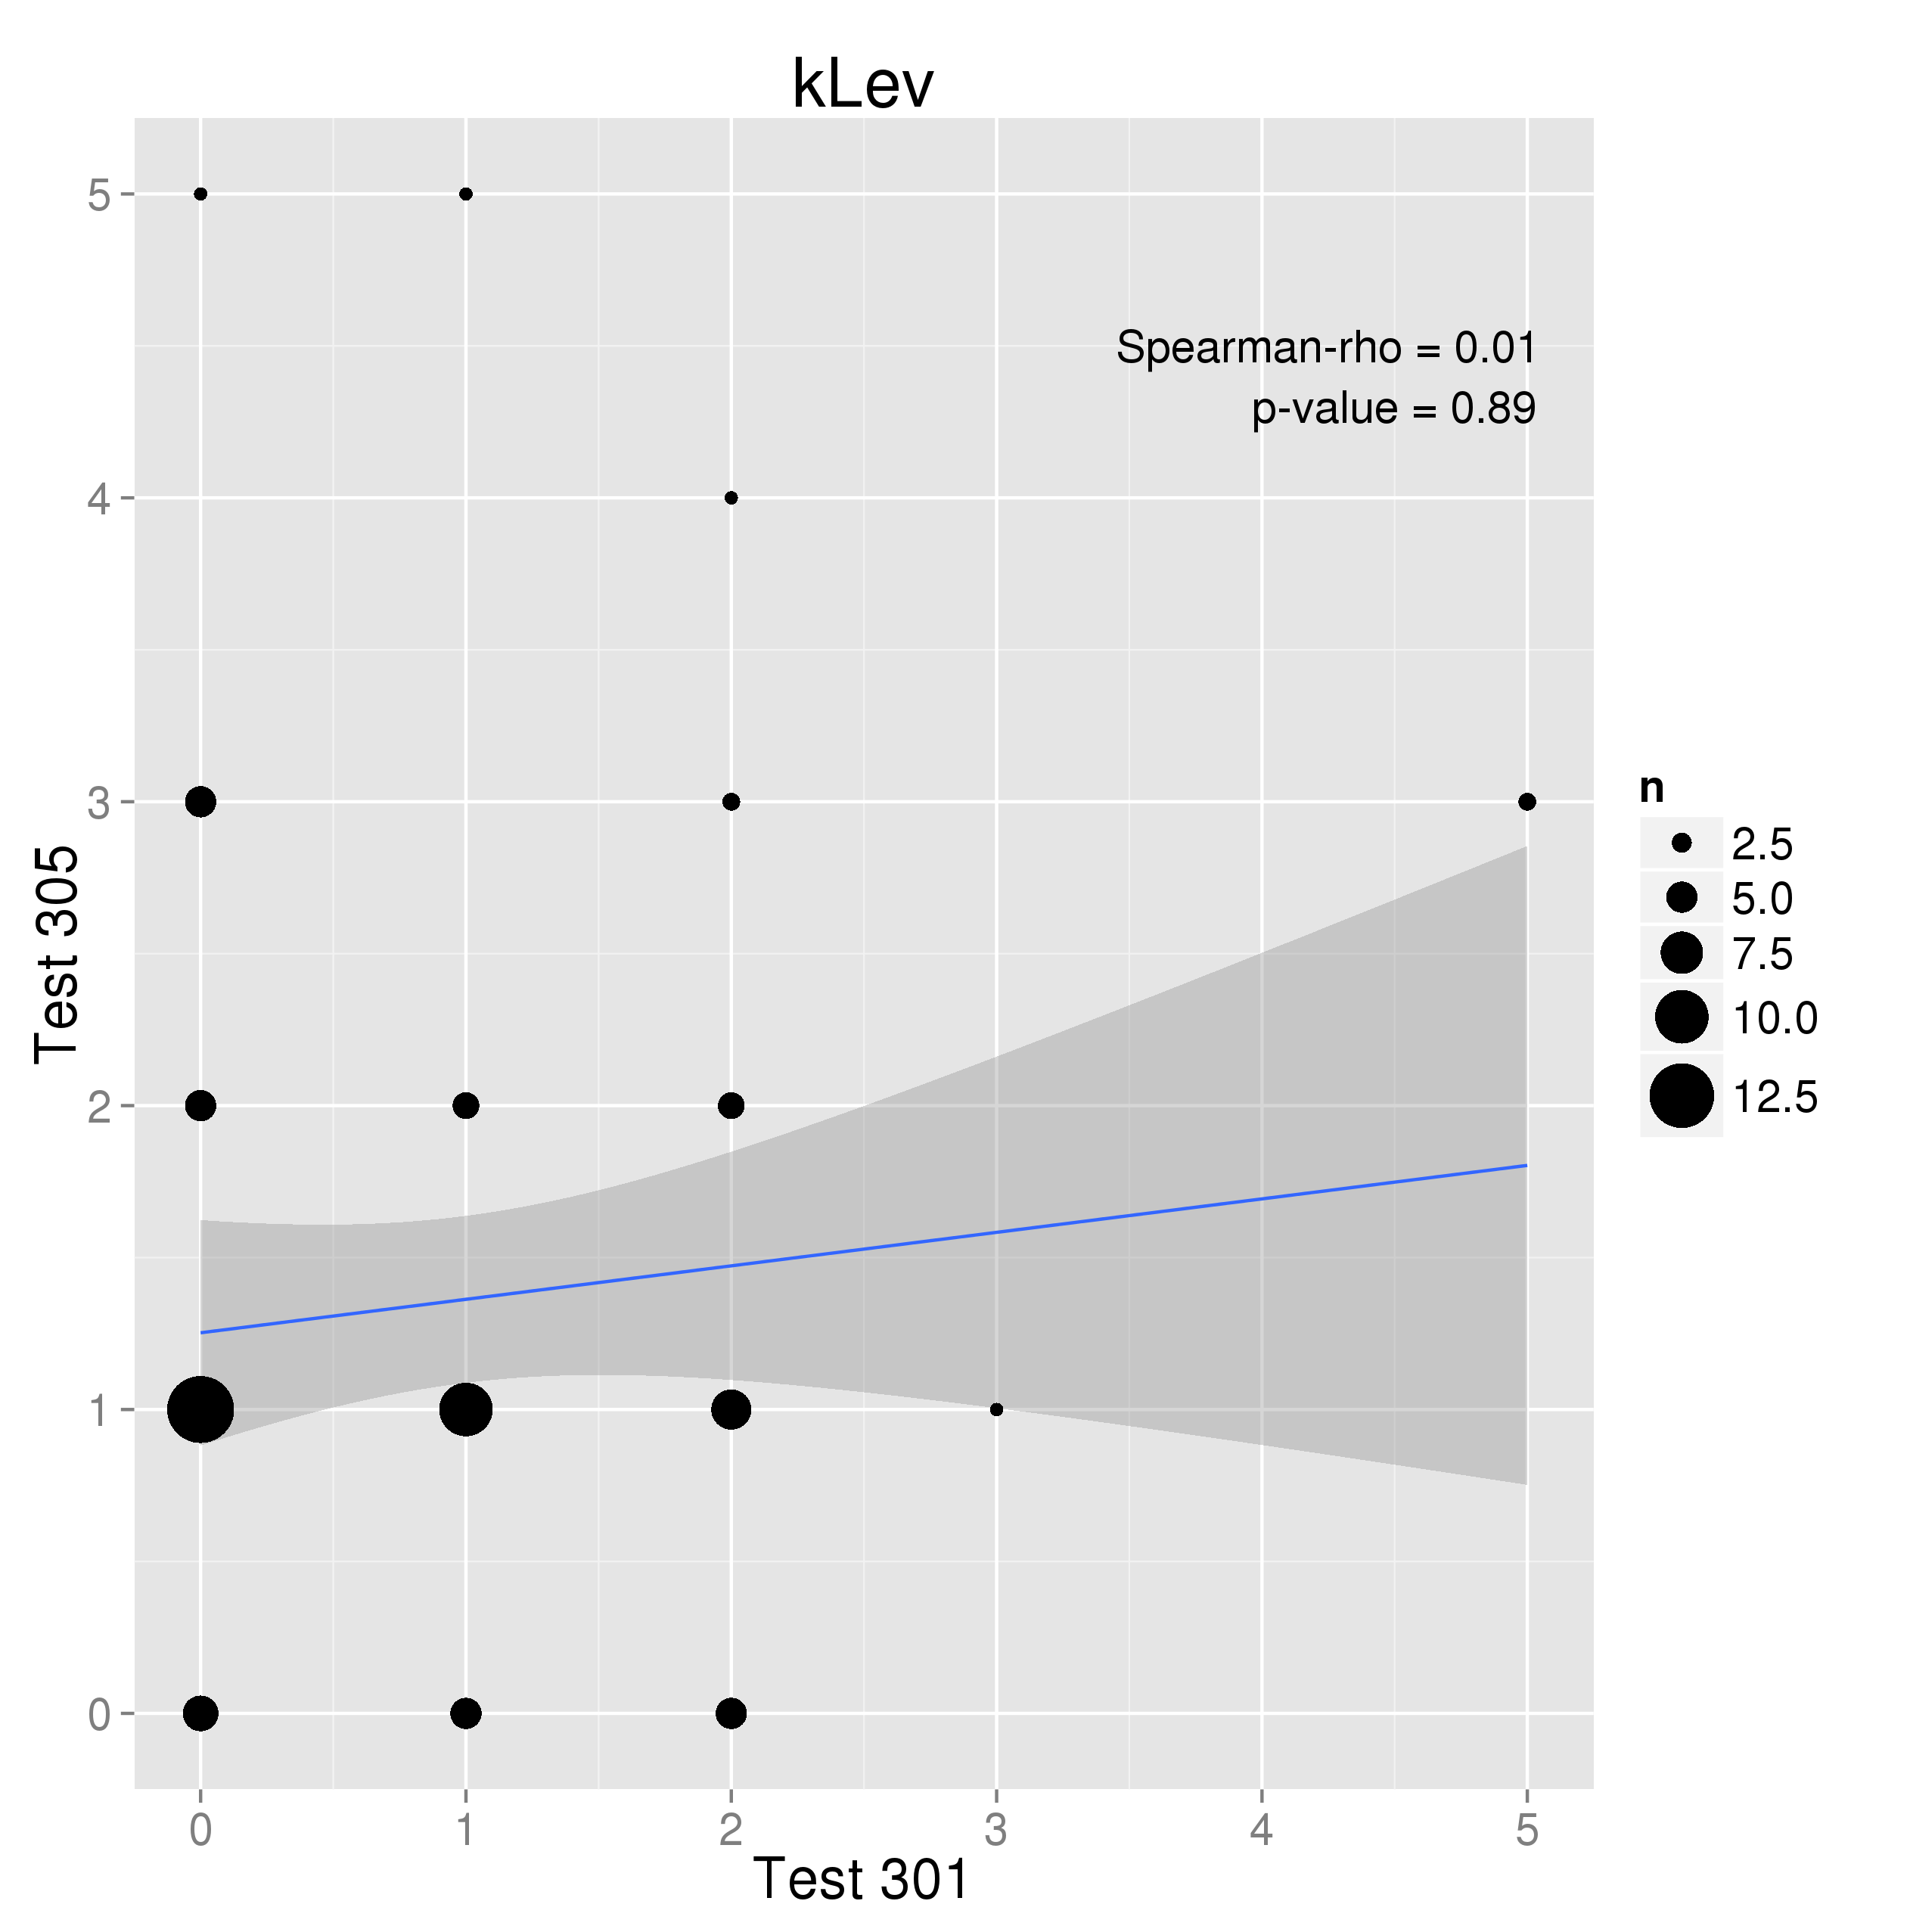
\includegraphics[width=1.0\linewidth]{graphics/cor301305k.png}
  \caption{bedingte Niveau-Stufen}
  \label{fig:cor301305u}
\end{subfigure}

\caption{Korrelation zwischen den Niveau Stufen zwischen den einzelnen Tests. Der Durchmesser der Punkte ist ein Mass für die Anzahl an Datenpunkten, welche an dieser Position liegen. Die blaue Gerade ist die lineare Regression der zugrunde liegenden Daten, der dunkel graue Bereich stellt das Vertrauensintervall (95\%) der linearen Regression dar. Zusätzlich sind noch Spearmans $rho$ und der p-Wert des Signifikanztests angegeben.}
\label{fig:corLev}
\end{figure}

\github{http://git.io/FnbD}


\section{Rasch-Analyse}

Als Probabilistische Test-Methode wurde das Rasch Modell verwendet. Der Grund für diese Methodik war, dass es sich bei der Kompetenz des skalenbasierten Messens um ein latentes Merkmal handelt. In anderen Worten die Kompetenz des skalenbaiserten Messens ist nicht direkt beobachtbar.

Es wurde zuerst folgendes Rasch Modell verwendet.

\begin{eqnarray}
P(U_{ij}=u_{ij}|\theta_i,\beta_j) = \frac{e^{u_{ij}(\theta_i-\beta_j)}}{1+e^{\theta_i-\beta_j}}
\end{eqnarray}

Wobei i=1,…,n die Zählvariable für eine Person ist und j=1,…,m die Zählvariable für eine Aufgabe darstellt. Die Variable $u_{ij} \in \{0,1\}$ die dichotome Antwort einer Person auf eine Frage ist. Die Variable $\beta_j$ beschreibt den Schwierigkeitsgrad einer Aufgabe und $\theta_j$ die latente Fähigkeit einer Person.

Bei der Item-Response-Theorie (Probabilistische Test-Methoden) wird angenommen , dass das Ergebnis einer Person nicht deterministisch ist, sondern zufällig sein kann. Daher soll mit dem Rasch Modell die Lösungswahrscheinlichkeit jeder Aufgabe $U_{ij}$ berechnet werden. Diese Lösungswahrscheinlichkeit hängt sowohl von der Fähigkeit der Person $\theta_j$ als auch von der Schwierigkeit der Aufgabe $\beta_i$ ab. Diese Lösungswahrscheinlichkeiten werden basierend auf den Testergebnissen $u_{ij}$ geschätzt.

\subsection{Parameterschätzung}
Für die Parameterschätzung gibt es verschieden Ansätze. Da die beste Methode von den Daten abhängig ist wurde in einem ersten Schritt das Rasch-Modell sowohl mit der bedingte Maximum-Likelihood-Schätzung, als auch mit der marginal Maximum-Likelihood-Schätzung getestet und die Resultate wurden verglichen. 

Bei der bedingten Maximum-Likelihood-Schätzung wird ein zweistufiges Vorgehen gewählt. Zuerst werden die Aufgaben-Parameter geschätzt ohne die Personen Parameter zu beachten. Erst in einem zweiten Schritt werden die Personen-Parameter geschätzt. Ein Problem dieser Methodik ist, dass Personenfertigkeiten von Personen, welche keine oder alle Aufgaben gelöst haben nicht geschätzt werden können \citep{Mair2007}.

In der marginalen Maximum-Likelihood-Schätzung wird angenommen, dass für die Personenfähigkeiten in der Stichprobe eine Normalverteilung vorliegt. Diese Annahme ist insbesondere dann problematisch, wenn nur eine Stichprobe der Gesamtbevölkerung verwendet wird \citep{Rizopoulos2006}.

Da beide Schätzungen für den vorliegenden Datensatz problematisch sein könnten, wurde das Rasch-Modell mit beiden Ansätzen durchgeführt und die Resultate verglichen. Das Ziel war dabei, den besseren Ansatz für den vorliegenden Datensatz zu finden, um mit diesem Ansatz die weiteren Analysen durchzuführen. Als Datensatz für diesen Vergleich wurden die 15 unbedingten Qualitätsstandards verwendet. Die Resultate sind in Abbildung \ref{fig:RaschVergleich} ersichtlich. Es gibt für diesen Datensatz keinerlei Unterschied in beiden Parameterschätzern.


\begin{figure}[htbp]

\centering
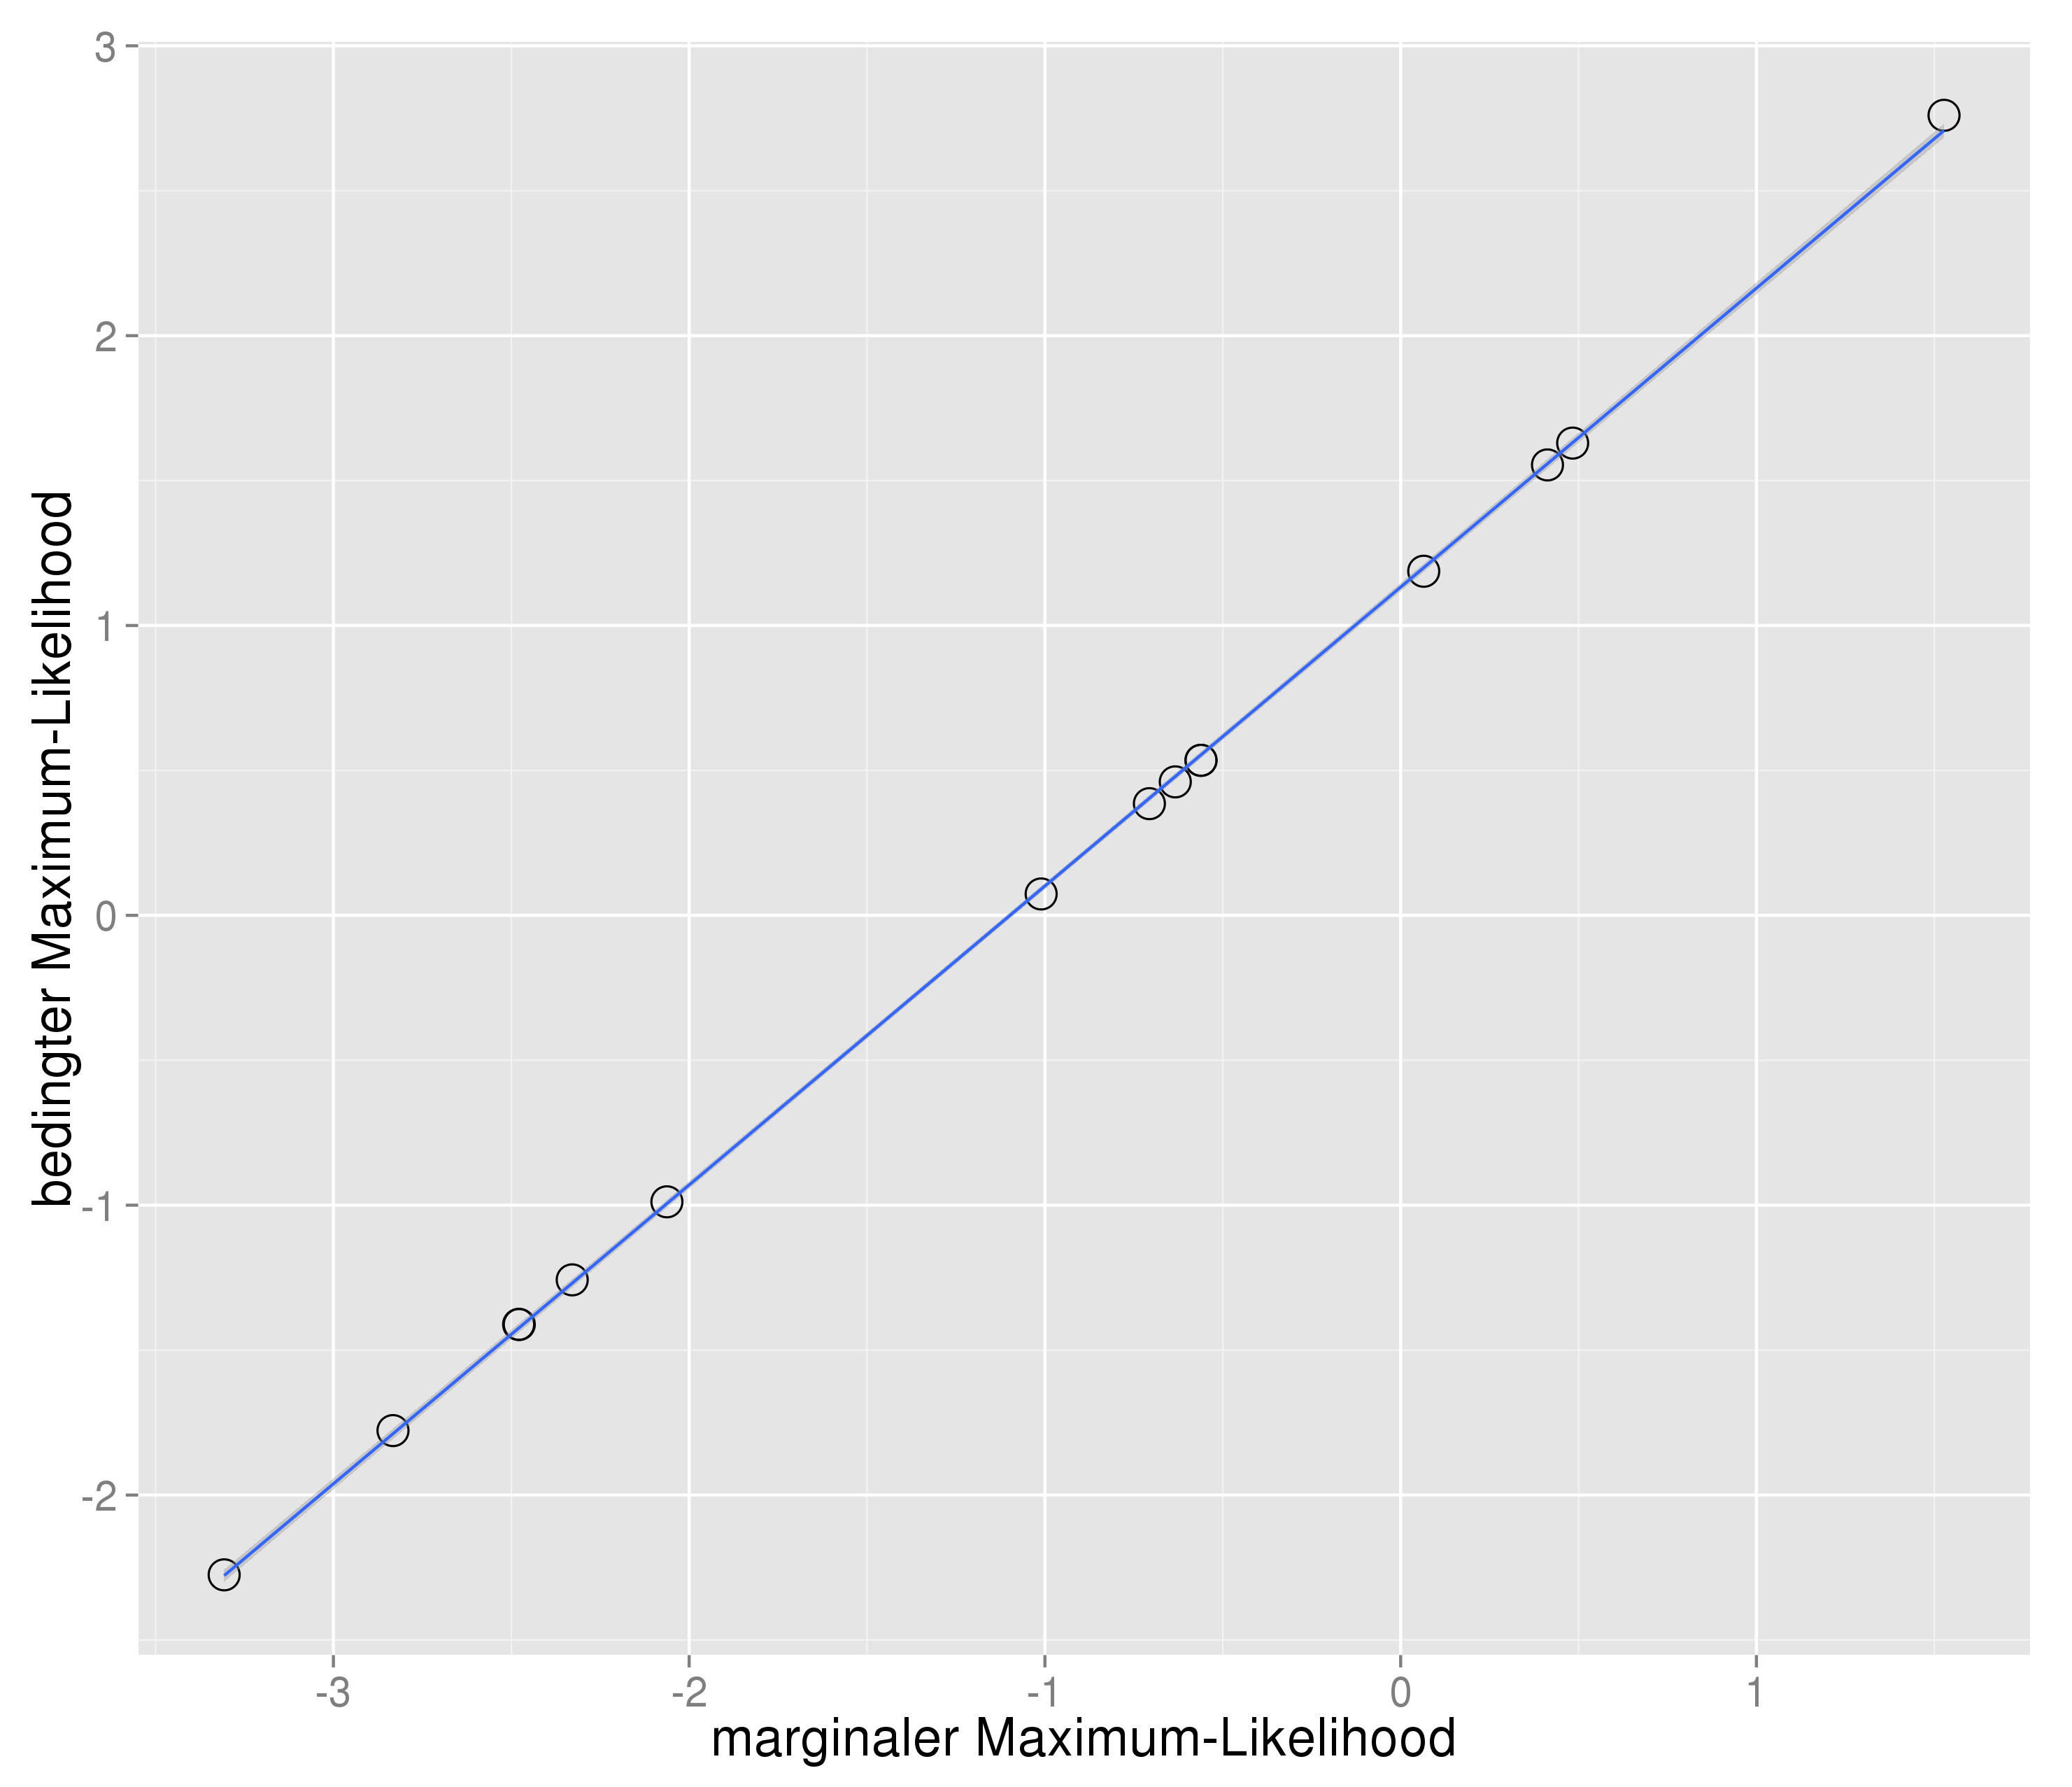
\includegraphics[width=0.7\linewidth]{graphics/RaschVergleich.png}
\caption{Vergleich des Rasch Modells mit der bedingten Maximum-Likelihood-Schätzung und der marginalen Maximum-Likelihood-Schätzung. Da alle Punkte auf einer Geraden liegen, gibt es keinen Unterschied zwischen den unterschiedlichen Schätzmethoden für den vorliegenden Datensatz der 15 unbedingten Qualitätsstandards.  }
\label{fig:RaschVergleich}
\end{figure}

\github{http://git.io/FRxZ}


\subsection{Modellkontrolle des Rasch-Modells}

Um das Rasch Modell zu Validieren wurde das Modell mit Hilfe des Andersens Likelihood-Quotienten Test validiert. Für alle 15 Qualitätsstufen führte dies zu Problemen und der Test konnte nicht durchgeführt werden. Nachdem die Qualitätsstufen vier und fünf entfernt wurden, konnte das reduzierte Modell validiert werden. Als Splitkriterium wurde der Mittelwert der Personen-Randsummen verwendet. 

Der p-Wert des Andersens Likelihood-Quotienten Test beträgt $p=0.14$. Daher liegt jetzt keine signifikante Modellverletzung vor, die Aufgaben Parameter unterscheiden sich nicht signifikant für Personen mit niedrigen und hohen Randsummen. In der Grafik \ref{fig:RaschKontrolle} sind die Resultate des Tests grafisch dargestellt. Es ist ersichtlich, dass keine Aufgabe das Modell verletzt, da die 95\%-Konfidenz-Regionen alle die Diagonale berühren.


\begin{figure}[htbp]

\centering
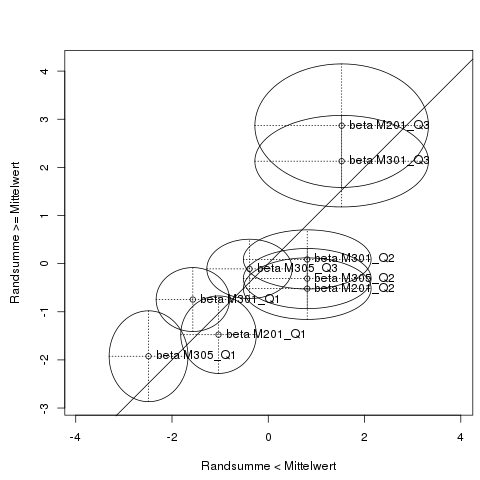
\includegraphics[width=0.8\linewidth]{graphics/GOFQ.png}
\caption{Modellkontrolle des Rasch-Modells: kein Qualitätsstandard hat eine signifikante Abweichung von der Diagonalen, daher gibt es keine signifikanten Unterschiede für Personen mit niedrigen und hohen Randsummen in den Qualitätsstandard. }
\label{fig:RaschKontrolle}
\end{figure}

Zusätzlich wurden die Qualitätsstandards mit dem Wald-Test überprüft. Damit können Qualitätsstandard, welche einen signifikanten Unterschied habe, identifiziert werden. In Tabelle \ref{tab:WaldTest} befinden sich die p-Werte des Wald-Test für die einzelnen Qualitätsstandards.

\begin{table}[htbp]
  \centering
\begin{tabular}{ccccccccccc}
\toprule
 \multicolumn{3}{c}{Test 201} &&  \multicolumn{3}{c}{Test 301}&&  \multicolumn{3}{c}{Test 305}\\ 
 Q1 & Q2 & Q3 && Q1 & Q2 & Q3 && Q1 & Q2 & Q3  \\ 
\midrule
  0.44 & 0.08 & 0.24 && 0.11 & 0.33 & 0.56 && 0.38 & 0.14 & 0.61   \\ 

\bottomrule
\end{tabular} 
  \caption{p-Werte des Wald-Tests für die Qualitätsstandards, mit dem Mittelwert der Personen-Randsummen als Splitkriterium. Keine dieser p-Werte liegt unter halb von $0.05$ daher gibt es keine signifikanten Unterschiede in den Qualitätsstandards }
  \label{tab:WaldTest}
\end{table}

\github{http://git.io/FE3m}

\subsection{Unterschied in den Qualitätsstandards}

Nachdem das Modell kontrolliert wurde soll nun überprüft werden ob es einen Unterschied in den Qualitätsstandards zwischen den einzelnen Test gibt.


  
 \begin{figure}[htp]
 \centering
 \begin{subfigure}{0.49\textwidth}
   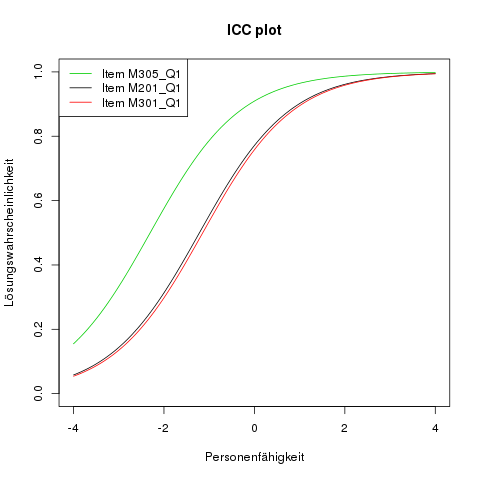
\includegraphics[width=1.0\linewidth]{graphics/ICCQ1.png}
   \caption{ICC Plot für Qualitätsstandard 1}
   \label{fig:ICCQ1}
 \end{subfigure}
 \begin{subfigure}{0.49\textwidth}
   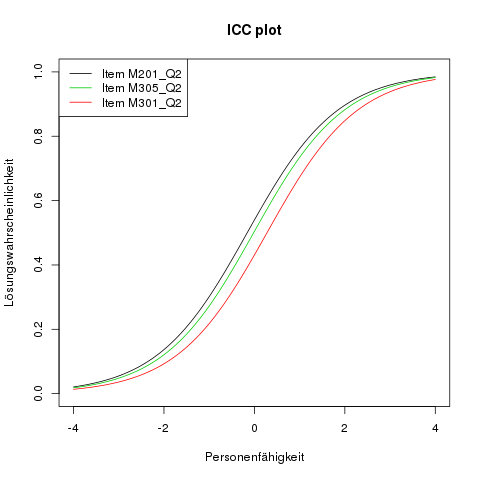
\includegraphics[width=1.0\linewidth]{graphics/ICCQ2.png}
   \caption{ICC Plot für Qualitätsstandard 2}
   \label{fig:ICCQ2}
 \end{subfigure}
 \end{figure}
 \begin{figure}[htbp]
 \ContinuedFloat % continue from previous page
 \centering
 \begin{subfigure}{0.49\textwidth}
   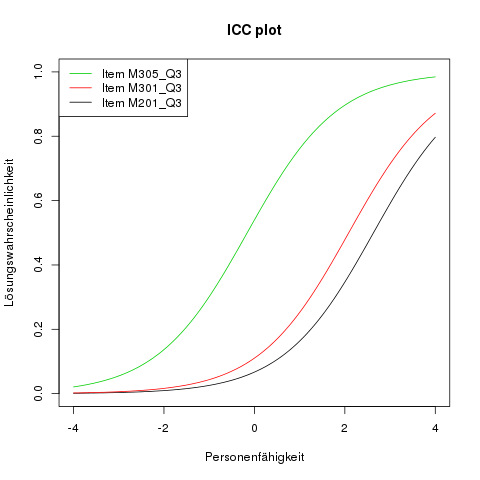
\includegraphics[width=1.0\linewidth]{graphics/ICCQ3.png}
   \caption{ICC Plot für Qualitätsstandard 3}
   \label{fig:ICCQ3}
 \end{subfigure}
 \begin{subfigure}{0.49\textwidth}
   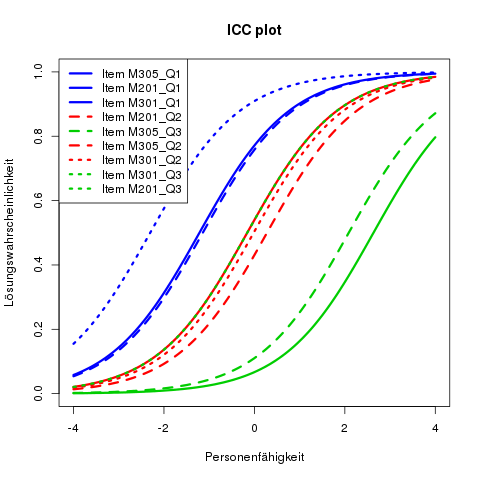
\includegraphics[width=1.0\linewidth]{graphics/ICCQ123.png}
   \caption{ICC Plot für Qualitätsstandard 1,2 und 3}
   \label{fig:ICCQ123}
 \end{subfigure}
 
 \caption{Aufgabencharakteristische Kurven für die Qualitätsstandards 1,2 und 3 für alle drei Tests.}
 \label{fig:corLev}
 \end{figure}
 
 \begin{figure}[htbp]
 
 \centering
 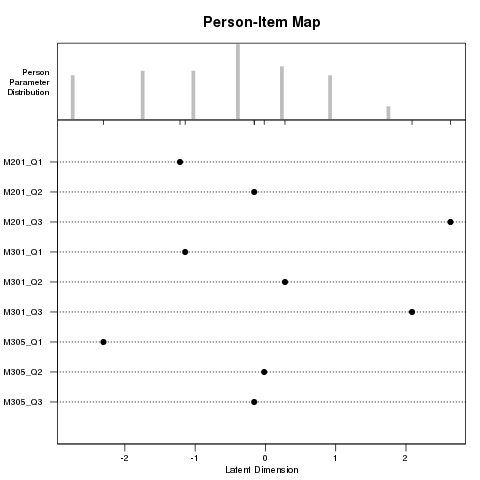
\includegraphics[width=0.8\linewidth]{graphics/PersonItemMap.png}
 \caption{Person-Item-Map auf welcher die Verteilung der Personen basierend auf der latenten Skala ersichtlich ist und die Lage der Aufgaben-Parameter auf der latenten Skala. }
 \label{fig:PersonItemMapQ}
 \end{figure}
 
 In Tabelle \ref{tab:betaQ} finden sich die Aufgaben-Parameter $\beta_j$ der einzelnen Qualitätsstandards.
 
 \begin{table}[htbp]
   \centering
 \begin{tabular}{ccccccccccc}
 \toprule
  \multicolumn{3}{c}{Test 201} &&  \multicolumn{3}{c}{Test 301}&&  \multicolumn{3}{c}{Test 305}\\ 
  Q1 & Q2 & Q3 && Q1 & Q2 & Q3 && Q1 & Q2 & Q3  \\ 
 \midrule
   1.215 & 0.159 & -2.633 && 1.142 & -0.278 & -2.086 && 2.305 & 0.017 & 0.159   \\ 
 
 \bottomrule
 \end{tabular} 
   \caption{Aufgaben-Parameter $\beta_j$ für die einzelnen Qualitätsstandards. }
   \label{tab:betaQ}
 \end{table}
\chapter{Diskussion}

\chapter{Ausblick}

\nocite{Gut2013a}
\nocite{Metzger2013}
\appendix 



\backmatter	

\printbibliography[heading=bibintoc]

\chapter{Anhang}

\end{document}
